\documentclass[letterpaper,12pt]{report}

\usepackage{thesis}

%\usepackage[pdftex,colorlinks=true,linkcolor=black,citecolor=black,filecolor=black,urlcolor=black,pdftitle={\xtitle},pdfauthor={\xauthor},pdfkeywords={\xkeywords},pdfsubject={\xsubject}]{hyperref} %

% Our stuff to set chapters, page size etc
%\usepackage{Setup/avlthesis}
% Our stuff to set math defs etc
%\usepackage{Setup/avldefs}   
% My stuff to set very personal defs
%\usepackage{Setup/mydefs}  


\usepackage{setspace}
\doublespacing

%\usepackage{fullpage}
\usepackage[sort&compress,square,comma,authoryear]{natbib}


%% The amssymb package provides various useful mathematical symbols
\usepackage{amssymb}
\usepackage{bm} 
\usepackage{graphicx}
\usepackage{float}
\usepackage{wrapfig}

%\usepackage{nomencl}
\usepackage{amsmath}
\usepackage{verbatim}
\usepackage{subfig}
\usepackage{epsfig}
\usepackage{subfig}
\usepackage{tikz}
\usetikzlibrary{snakes}
\usepackage{pstricks}
\usepackage{url}
%\usepackage{nomencl}
\usepackage{mathtools}
\usepackage{algorithm}
\usepackage{algorithmic}
\usepackage{enumitem}% http://ctan.org/pkg/enumitem
\usepackage{IEEEtrantools}
\usepackage{pifont}% http://ctan.org/pkg/pifont
\newcommand{\cmark}{\ding{51}}%
\newcommand{\xmark}{\ding{55}}%

\def\red{\textcolor[rgb]{0,0,0}}
\def\green{\textcolor[rgb]{0,0,0}}

% Title is overwritten in title.tex
\def\xtitle{A finite element method for linear and non-linear poroelasticity: theory and application to lung modelling}
%A Computational Investigation of Acute Ischaemia-induced Changes in Cardiac Electrophysiology: From Rabbit Experiments to Drug Safety in Human
\def\xauthor{Lorenz Berger}
\def\xcollege{Keble College}
\def\xterm{Michaelmas Term 2014}
\def\xkeywords{some keywords}
\def\xsubject{a subject}


\newenvironment{abstractchap}{\rightskip1in\itshape}{}


%Defines
%\input{/users/lorenzb/Dphil/poroelasticity_papers/coupling_paper/contents/defines}
%%%%%%%%%%%%%%%%%%%%%%%%%%%%%%%%%%%%%%%%%%%%%%%%%%%%%%%%%%%%%%%%%%%%%%%%%%%%%%%%%%%%%%%%%%%%%%%%%%%%%
%                                           VARIABLES                                              %
%%%%%%%%%%%%%%%%%%%%%%%%%%%%%%%%%%%%%%%%%%%%%%%%%%%%%%%%%%%%%%%%%%%%%%%%%%%%%%%%%%%%%%%%%%%%%%%%%%%%

%Displacement
\newcommand{\dispcont}{\mathbf{u}}
\newcommand{\dispcontn}{\mathbf{u}(t_{n}, \cdot)}
\newcommand{\dispconttest}{\mathbf{v}}
\newcommand{\dispconttime}{{\mathbf{u}_{t}}}
\newcommand{\dispconttimen}{{\mathbf{u}_{t}}(t_{n},\cdot)}
\newcommand{\dispconttimedisc}{{\mathbf{u}_{\Delta t}}}
\newcommand{\dispconttimediscn}{{\mathbf{u}_{\Delta t}}(t_{n},\cdot)}
\newcommand{\dispdisctimediscn}{{\mathbf{u}_{\Delta t,h}^{n}}}
\newcommand{\dispdisctimen}{{\boldsymbol{u}^{n}_{h, \Delta t}}}

\newcommand{\dispdisc}{\mathbf{u}_{h}}
\newcommand{\dispdiscn}{\mathbf{u}_{h}^{n}}
\newcommand{\dispdisctest}{\mathbf{v}_{h}}
\newcommand{\dispdisctime}{{\mathbf{u}_{t}}_{h}}
\newcommand{\dispdisctimedisc}{{\mathbf{u}_{\Delta t,h}}}

%Fluid flux
\newcommand{\fluxcont}{\mathbf{z}}
\newcommand{\fluxcontn}{\mathbf{z}(t_{n},\cdot)}
\newcommand{\fluxconttest}{\mathbf{w}}
\newcommand{\fluxconttime}{\mathbf{z}_{t}}
\newcommand{\fluxconttimen}{\mathbf{z}_{t}(t_{n},\cdot)}
\newcommand{\fluxconttimedisc}{\mathbf{z}_{\Delta t}}
\newcommand{\fluxconttimediscn}{\mathbf{z}_{\Delta t}(t_{n})}

\newcommand{\fluxdisc}{\mathbf{z}_{h}}
\newcommand{\fluxdiscn}{\mathbf{z}_{h}^{n}}
\newcommand{\fluxdisctest}{\mathbf{w}_{h}}
\newcommand{\fluxdisctime}{{\mathbf{z}_{t}}_{h}}
\newcommand{\fluxdisctimedisc}{{\mathbf{z}_{\Delta t,h}}}
\newcommand{\fluxdisctimediscn}{{\mathbf{z}_{\Delta t,h}^{n}}}


%Pressure
\newcommand{\pcont}{p}
\newcommand{\pcontn}{p(t_{n},\cdot)}
\newcommand{\pconttest}{{q}}
\newcommand{\pconttime}{{{p}_{t}}}
\newcommand{\pconttimen}{{{p}_{t}}(t_{n},\cdot)}
\newcommand{\pconttimedisc}{{{p}_{\Delta t}}}
\newcommand{\pconttimediscn}{{{p}_{\Delta t}}(t_{n}, \cdot)}
\newcommand{\pconthat}{\hat{p}}

\newcommand{\pdisc}{p_h}
\newcommand{\pdiscn}{p_{h}^{n}}
\newcommand{\pdisctest}{{q}_{h}}
\newcommand{\pdisctime}{{{p}_{t}}_h}
\newcommand{\pdisctimedisc}{{{p}_{\Delta t,h}}}
\newcommand{\pdisctimediscn}{{{p}_{\Delta t,h}^{n}}}
\newcommand{\pdischat}{\hat{p}_h}


%Other variables
\newcommand{\normal}{\mathbf{n}}
\newcommand{\proj}{\pi_{h}^{OLD}}
\newcommand{\projconst}{\pi_{h}^{0}}
\newcommand{\projlinear}{\pi_{h}^{1}}
\newcommand{\projscott}{\pi_{h}^{1}}%%{\pi_{h}^{s}}
\newcommand{\vp}{\mathbf{v}_{p}}
\newcommand{\vph}{\mathbf{v}_{p_h}}
\newcommand{\vphn}{\mathbf{v}_{p_h^n}}
\newcommand{\vthetadtn}{\mathbf{v}_{\theta_{\Delta t, p}^n}}

\newcommand{\fdispcont}{\mathbf{r}}
\newcommand{\fdispconttime}{\mathbf{r}_{t}}


%%%%%%%%%%%%%%%%%%%%%%%%%%%%%%%%%%%%%%%%%%%%%%%%%%%%%%%%%%%%%%%%%%%%%%%%%%%%%%%%%%%%%%%%%%%%%%%%%%%%
%                                             SPACES                                               %
%%%%%%%%%%%%%%%%%%%%%%%%%%%%%%%%%%%%%%%%%%%%%%%%%%%%%%%%%%%%%%%%%%%%%%%%%%%%%%%%%%%%%%%%%%%%%%%%%%%%

%Continuous spaces
\newcommand{\dispspace}{\mathbf{W}^{E}(\Omega)}
\newcommand{\fluxspace}{\mathbf{W}^{D}(\Omega)}
\newcommand{\pspace}{\mathcal{L}(\Omega)}

%Discrete spaces
\newcommand{\dispspacedisc}{\mathbf{W}^{E}_{h}}
\newcommand{\fluxspacedisc}{\mathbf{W}^{D}_{h}}
\newcommand{\pspacedisc}{{Q}_{h}}
\newcommand{\pspacedisctest}{{Q}_{h}}

% Test spaces
\newcommand{\elastspacetest}{\mathbf{W}^{E}_{0}(\Omega)}
\newcommand{\darcyspacetest}{\mathbf{W}^{D}_{0}(\Omega)}
\newcommand{\pspaceconttest}{\mathcal{L}(\Omega)}


%Mixed spaces
\newcommand{\mixedspace}{\mathcal{W}^{X}}
\newcommand{\mixedspacetime}{\mathcal{W}^{X}_{T}}
\newcommand{\mixedspacedisc}{\mathcal{W}^{X}_{h}}
\newcommand{\mixedspacedisctau}{\mathcal{W}^{X}_{\tau\, h}}

\newcommand{\dispspacedisctest}{\mathbf{W}^{E}_{h0}}
\newcommand{\fluxspacedisctest}{\mathbf{W}^{D}_{h0}}

\newcommand{\mixedspacetest}{\mathcal{V}^{X}}
\newcommand{\mixedspacedisctest}{\mathcal{V}^{X}_{h}}

\newcommand{\honespace}{\left[ H^{1}_{0}  \right]^{d}}
\newcommand{\polyspace}{\mathbf{V}_{h}}




%%%%%%%%%%%%%%%%%%%%%%%%%%%%%%%%%%%%%%%%%%%%%%%%%%%%%%%%%%%%%%%%%%%%%%%%%%%%%%%%%%%%%%%%%%%%%%%%%%%%
%                                           ERRORS                                                 %
%%%%%%%%%%%%%%%%%%%%%%%%%%%%%%%%%%%%%%%%%%%%%%%%%%%%%%%%%%%%%%%%%%%%%%%%%%%%%%%%%%%%%%%%%%%%%%%%%%%%

%Auxiliary errors
\newcommand{\auxdisp}{\mathbf{\theta}_{\mathbf{u}}}
\newcommand{\auxdispn}{\mathbf{\theta}^{n}_{\mathbf{u}}}
\newcommand{\auxdispntime}{\mathbf{\theta}^{n}_{\Delta t ,\mathbf{u}}}
\newcommand{\auxdisptime}{\mathbf{\theta}_{\Delta t ,\mathbf{u}}}
\newcommand{\auxdispnm}{\mathbf{\theta}^{n-1}_{\mathbf{u}}}

\newcommand{\auxflux}{\mathbf{\theta}_{\mathbf{z}}}
\newcommand{\auxfluxn}{\mathbf{\theta}^{n}_{\mathbf{z}}}
\newcommand{\auxfluxntime}{\mathbf{\theta}^{n}_{\Delta t, \mathbf{z}}}

\newcommand{\auxp}{{\theta}_{{p}}}
\newcommand{\auxpn}{{\theta}^{n}_{{p}}}
\newcommand{\auxpntime}{{\theta}^{n}_{\Delta t, p}}
\newcommand{\auxptime}{{\theta}_{\Delta t, p}}

\newcommand{\auxphat}{{\theta}_{{\hat{p}}}}
\newcommand{\auxpnhat}{{\theta}^{n}_{{\hat{p}}}}

%Interpolation errors
\newcommand{\intdisp}{\mathbf{\eta}_{\mathbf{u}}}
\newcommand{\fedisp}{\mathbf{e}_{\mathbf{u}}}
\newcommand{\feflux}{\mathbf{e}_{\mathbf{z}}}
\newcommand{\fep}{{e}_{{p}}}
\newcommand{\intdispn}{\mathbf{\eta}^{n}_{\mathbf{u}}}
\newcommand{\intdispntime}{\mathbf{\eta}^{n}_{\Delta t, \dispcont}}
\newcommand{\intdisptime}{\mathbf{\eta}_{\Delta t ,\dispcont}}
\newcommand{\intdispnconttime}{\mathbf{\eta}^{n}_{\dispcont_{t}}}
\newcommand{\intdispnconttimet}{\mathbf{\eta}^{n}_{\dispcont_{tt}}}
\newcommand{\intdispconttime}{\mathbf{\eta}_{\dispcont_{t}}}
\newcommand{\intdispconttimet}{\mathbf{\eta}_{\dispcont_{tt}}}

\newcommand{\intdispnt}{\mathbf{\eta}^{n}_{\mathbf{u}_{t}}}
\newcommand{\intdispntm}{\mathbf{\eta}^{n-1}_{\mathbf{u}_{t}}}
\newcommand{\intdispnm}{\mathbf{\eta}^{n-1}_{\mathbf{u}}}

\newcommand{\intfluxn}{\mathbf{\eta}^{n}_{\mathbf{z}}}
\newcommand{\intflux}{\mathbf{\eta}_{\mathbf{z}}}
\newcommand{\intfluxntime}{\mathbf{\eta}^{n}_{\Delta t ,\fluxcont}}
\newcommand{\intfluxtime}{\mathbf{\eta}_{\Delta t ,\fluxcont}}
\newcommand{\intfluxconttime}{\mathbf{\eta}_{\fluxcont_{t}}}
\newcommand{\intfluxconttimet}{\mathbf{\eta}_{\fluxcont_{tt}}}

\newcommand{\intpn}{{\eta}^{n}_{{p}}}
\newcommand{\intpnm}{{\eta}^{n-1}_{{p}}}
\newcommand{\intpntime}{{\eta}^{n}_{\Delta t ,\pcont}}
\newcommand{\intptime}{{\eta}_{\Delta t ,\pcont}}
\newcommand{\intpnhat}{{\eta}^{n}_{{{p}}}}
\newcommand{\intpnconttime}{{\eta}^{n}_{\pcont_{t}}}
\newcommand{\intpconttime}{{\eta}_{\pcont_{t}}}
\newcommand{\intpnconttimet}{{\eta}^{n}_{\pcont_{tt}}}
\newcommand{\intpconttimet}{{\eta}_{\pcont_{tt}}}

%Time errors
\newcommand{\timerr}{\mathbf{\rho}}
\newcommand{\disptimerrn}{\mathbf{\rho}_{\dispcont}^{n}}
\newcommand{\ptimerrn}{{\rho}_{\pcont}^{n}}

%Other errors
\newcommand{\edisp}{\mathbf{e_{u}}}
\newcommand{\eflux}{\mathbf{e_{z}}}
\newcommand{\ep}{{e_{p}}}
\newcommand{\dispinterp}{\mathbf{\eta}_{u}}
\newcommand{\disptinterp}{\mathbf{\eta}_{u_{t}}}


%%%%%%%%%%%%%%%%%%%%%%%%%%%%%%%%%%%%%%%%%%%%%%%%%%%%%%%%%%%%%%%%%%%%%%%%%%%%%%%%%%%%%%%%%%%%%%%%%%%%
%                                       TRIPLE NORMS                                               %
%%%%%%%%%%%%%%%%%%%%%%%%%%%%%%%%%%%%%%%%%%%%%%%%%%%%%%%%%%%%%%%%%%%%%%%%%%%%%%%%%%%%%%%%%%%%%%%%%%%%

%Abreviation for triples
\newcommand{\conttriple}{(\dispcont,\fluxcont,\pcont)}
\newcommand{\conttriplehat}{(\dispcont,\fluxcont,\pconthat)}

\newcommand{\conttripletest}{(\dispconttest,\fluxconttest,\pconttest)}
\newcommand{\disctriple}{(\dispdisc,\fluxdisc,\pdisc)}
\newcommand{\disctriplehat}{(\dispdisc,\fluxdisc,\pdischat)}

\newcommand{\disctriplen}{(\dispdisc^{n},\fluxdisc^{n},\pdisc^{n})}
\newcommand{\disctriplenhat}{(\dispdisc^{n},\fluxdisc^{n},\pdischat^{n})}

\newcommand{\conttriplen}{(\dispcontn,\fluxcontn,\pcontn)}
\newcommand{\conttriplenhat}{(\dispcont^{n},\fluxcont^{n},\pconthat^{n})}

\newcommand{\errortriplen}{(\dispcontn-\dispdisc^{n},\fluxcontn-\fluxdisc^{n},\pcontn-\pdisc^{n})}
\newcommand{\feerrortriplen}{(\fedisp^{n},\feflux^{n},\fep^{n})}
\newcommand{\feerrortriple}{(\fedisp,\feflux,\fep)}
\newcommand{\errortriplenhat}{(\dispcont^{n}-\dispdisc^{n},\fluxcont^{n}-\fluxdisc^{n},\pconthat^{n}-\pdischat^{n})}


\newcommand{\disctripletest}{(\dispdisctest,\fluxdisctest,\pdisctest)}
\newcommand{\disctripletesttime}{(\dispdisctest,\fluxdisctest,\pdisctest)}
\newcommand{\disctripletestn}{(\dispdisctest^{n},\fluxdisctest^{n},\pdisctest^{n})}

\newcommand{\errortriple}{(\dispcont-\dispdisc,\fluxcont-\fluxdisc,\pcont-\pdisc)}
\newcommand{\auxerrortriple}{(\mathbf{\eta},\mathbf{\omega},\zeta)}
\newcommand{\auxerrortriplen}{(\mathbf{\eta}^{n},\mathbf{\omega}^{n},\zeta^{n})}
\newcommand{\errortripletime}{(\dispcont-\dispdisc,\fluxcont-\fluxdisc,\pcont-\pdisc,\dispcont_{t}-\bar{\partial}{\dispdisc} )}



%%%%%%%%%%%%%%%%%%%%%%%%%%%%%%%%%%%%%%%%%%%%%%%%%%%%%%%%%%%%%%%%%%%%%%%%%%%%%%%%%%%%%%%%%%%%%%%%%%%%
%                                            NORMS                                                 %
%%%%%%%%%%%%%%%%%%%%%%%%%%%%%%%%%%%%%%%%%%%%%%%%%%%%%%%%%%%%%%%%%%%%%%%%%%%%%%%%%%%%%%%%%%%%%%%%%%%%

\newcommand{\seminorm}[1]      {{\left\vert #1 \right\vert}}

\newcommand{\doublenorm}[1]    {{\left\vert\kern-0.25ex\left\vert #1 \right\vert\kern-0.25ex\right\vert}}
\newcommand{\honenorm}[1]  {\doublenorm{#1}_{1,\Omega}}
\newcommand{\htwonorm}[1]  {\doublenorm{#1}_{2,\Omega}}
\newcommand{\htwonormk}[1] {\doublenorm{#1}_{2,K}}
\newcommand{\ltwonorm}[1]  {\doublenorm{#1}_{0,\Omega}}
\newcommand{\honenormk}[1] {\doublenorm{#1}_{1,K}}
\newcommand{\ltwonormk}[1] {\doublenorm{#1}_{0,K}}
\newcommand{\ltwonormdk}[1]{\doublenorm{#1}_{0,\partial K}}
\newcommand{\hmnorm}[1]    {\doublenorm{#1}_{m,\Omega}}
\newcommand{\dualnorm}[1]  {\doublenorm{#1}_{-1,\Omega}}

\newcommand{\triplenorm}[1]        {\left\vert\kern-0.25ex\left\vert\kern-0.25ex\left\vert #1 \right\vert\kern-0.25ex\right\vert\kern-0.25ex\right\vert_{A}}
\newcommand{\triplenormtime}[1]    {\left\vert\kern-0.25ex\left\vert\kern-0.25ex\left\vert #1 \right\vert\kern-0.25ex\right\vert\kern-0.25ex\right\vert_{B}}
\newcommand{\triplenormtimedisc}[1]{\left\vert\kern-0.25ex\left\vert\kern-0.25ex\left\vert #1 \right\vert\kern-0.25ex\right\vert\kern-0.25ex\right\vert_{B_{h,\Delta t}}}
\newcommand{\tripletimenorm}[1]    {{\left\vert\kern-0.25ex\left\vert\kern-0.25ex\left\vert #1 \right\vert\kern-0.25ex\right\vert\kern-0.25ex\right\vert}_{L^{2}}}

%
\newcommand{\anorm}[1] {\doublenorm{#1}_{a,\Omega}}
\newcommand{\jnorm}[1] {|{#1}|_{J,\Omega}}


%Time norms
\newcommand{\honetimenorm}[1]     {\doublenorm{#1}_{L^{2}(H^{1})}}
\newcommand{\htwotimenorm}[1]     {\doublenorm{#1}_{L^{2}(H^{2})}}
\newcommand{\ltwotimenorm}[1]     {\doublenorm{#1}_{L^{2}(L^{2})}}
\newcommand{\ltwotimecontnorm}[1] {\doublenorm{#1}_{L^{2}(L^{2})}}
\newcommand{\jtimenorm}[1]        {\doublenorm{#1}_{L^{2}(J)}}
\newcommand{\honetimeinftynorm}[1]{\doublenorm{#1}_{L^{\infty}(H^{1})}}
\newcommand{\htwotimeinftynorm}[1]{\doublenorm{#1}_{L^{\infty}(H^{2})}}
\newcommand{\ltwotimeinftynorm}[1]{\doublenorm{#1}_{L^{\infty}(L^{2})}}
\newcommand{\jtimeinftynorm}[1]   {\doublenorm{#1}_{L^{\infty}(J)}}

\newcommand{\honeconttimenorm}[1]{\doublenorm{#1}_{L^{2}(H^{1})}}
\newcommand{\htwoconttimenorm}[1]{\doublenorm{#1}_{L^{2}(H^{2})}}
\newcommand{\ltwoconttimenorm}[1]{\doublenorm{#1}_{L^{2}(L^{2})}}
\newcommand{\ltwoconttimeinftynorm}[1]{\doublenorm{#1}_{L^{\infty}(L^{2})}}

\newcommand{\jconttimenorm}[1]{\doublenorm{#1}_{L^{2}(J)}}

%Seminorms
\newcommand{\honeseminorm}[1]{\seminorm{#1}_{1,\Omega}}
\newcommand{\htwoseminorm}[1]{\seminorm{#1}_{2,\Omega}}
\newcommand{\jseminorm}[1]{\seminorm{#1}_{J,\Omega}}



%Theorems and Lemmas
%\newtheorem{theorem}{Theorem}[section]
%\newtheorem{lemma}[theorem]{Lemma}
%\newtheorem{proposition}[theorem]{Proposition}
%\newtheorem{corollary}[theorem]{Corollary}
%\newtheorem{remark}{Remark}



%%%%%%%%%%%%%%%%%%%%%%%%%%%%%%%%%%%%%%%%%%%%%%%%%%%%%%%%%%%%%%%%%%%%%%%%%%%%%%%%%%%%%%%%%%%%%%%%%%%%
%                                        MISCELLANEOUS                                             %
%%%%%%%%%%%%%%%%%%%%%%%%%%%%%%%%%%%%%%%%%%%%%%%%%%%%%%%%%%%%%%%%%%%%%%%%%%%%%%%%%%%%%%%%%%%%%%%%%%%%


%permeability tensor
\newcommand{\perm}{k}
\newcommand{\perminv}{k^{-1}}
%\newcommand{\permscalar}{{\kappa^{-1}}}
%\newcommand{\kperm}{\mathbf{k}_{f}}



%Shortenings.
\newcommand{\timederiv}{\frac{\partial }{\partial t }}

%Derivatives
\newcommand{\deriv}[2]{\frac{\mathrm{d}#1}{\mathrm{d}#2}}
\newcommand{\mderiv}[2]{\frac{\mathrm{D}#1}{\mathrm{D}#2}}
\newcommand{\pderiv}[2]{\frac{\partial #1}{\partial #2}}
\newcommand{\dderiv}[3]{\mbox{D} #1 (#2)[#3]}

%Spatial description of the material velocity
\newcommand{\vell}{\mathbf{v}(\mathbf{x},t)}
\newcommand{\vels}{\mathbf{v}}

%Material description of the material velocity
\newcommand{\Vell}{\mathbf{V}(\mathbf{X},t)}
\newcommand{\Vels}{\mathbf{V}}

%deformation map
\newcommand{\defmap}{\mathbf\varphi(\mathbf{X},t)}
\newcommand{\defmapinv}{\mathbf\varphi^{-1}(\mathbf{x},t)}

%spatial gradient
\newcommand{\spatgrad}{\nabla_{\mathbf{x}}}

%boldsymbol short
\newcommand{\bb}[1]{\mathbf{#1}}
%domega
\newcommand{\dv}{\mbox{d}\Omega}
%dbound
\newcommand{\ds}{\mbox{d}\Gamma}
%Gradients
\newcommand{\GradX}{\nabla_{\mathbf{X}}}
\newcommand{\gradx}{\nabla_{\mathbf{x}}}



%Helmholtz energy
\newcommand{\helm}{\mathbf{\Psi}}


%Tensors
\newcommand{\identity}{\mathbf{I}}
\newcommand{\spatialincremental}{\mathfrak{c}}
\newcommand{\si}{\mathfrak{c}}

%Divergence
\newcommand{\divergence}{\nabla \cdot}

%test functions for the dual problem (used to prove improved convergence)
\newcommand{\dispconttestd}{\mathbf{\phi}}
\newcommand{\fluxconttestd}{\mathbf{\psi}}
\newcommand{\pconttestd}{r}




\renewcommand{\mathbf}[1]{\boldsymbol{#1}}
\renewcommand{\citet}[1]{\cite{#1}}
\renewcommand{\citep}[1]{\cite{#1}}


%Derivatives
\newcommand{\deriv}[2]{\frac{\mathrm{d}#1}{\mathrm{d}#2}}
\newcommand{\mderiv}[2]{\frac{\mathrm{D}#1}{\mathrm{D}#2}}
\newcommand{\pderiv}[2]{\frac{\partial #1}{\partial #2}}
\newcommand{\dderiv}[3]{\mbox{D} #1 (#2)[#3]}
%Spatial description of the material velocity
\newcommand{\vell}{\mathbf{v}(\mathbf{x},t)}
\newcommand{\vels}{\mathbf{v}}

%Material description of the material velocity
\newcommand{\Vell}{\mathbf{V}(\mathbf{X},t)}
\newcommand{\Vels}{\mathbf{V}}

%deformation map
\newcommand{\defmap}{\mathbf\varphi(\mathbf{X},t)}
\newcommand{\defmapinv}{\mathbf\varphi^{-1}(\mathbf{x},t)}

%spatial gradient
\newcommand{\spatgrad}{\nabla_{\mathbf{x}}}

%boldsymbol short
\newcommand{\bb}[1]{\mathbf{#1}}
%domega
\newcommand{\dv}{\mbox{d}\Omega}
%dbound
\newcommand{\ds}{\mbox{d}\Gamma}
%Gradients
\newcommand{\Grad}{\nabla_{\mathbf{X}}}
\newcommand{\grad}{\nabla_{\mathbf{x}}}

%permeability tensor
\newcommand{\perm}{\mathbf{k}}
\newcommand{\perminv}{\mathbf{k^{-1}}}
\newcommand{\permscalar}{{k^{-1}}}
\newcommand{\kperm}{\mathbf{k}_{f}}

%Helmholtz energy
\newcommand{\helm}{\mathbf{\Psi}}

%Hoghlight questions
\def\quest{\textbf}

%colours
\def\green{\textcolor[rgb]{0,1,0}}
\def\red{\textcolor[rgb]{1,0,0}}
\def\blue{\textcolor[rgb]{0,0,1}}
\usepackage{xcolor}
\newcommand\hide[1]{\textcolor{red}{#1}}
\renewcommand\hide[1]{}

\newcommand\transfer[1]{\textcolor{red}{#1}}
\renewcommand\transfer[1]{}

%Tensors
\newcommand{\identity}{\mathbf{I}}
\newcommand{\spatialincremental}{\mathbf{\Theta}}
\newcommand{\si}{\mathbf{\Theta}}

%Divergence
\newcommand{\divergence}{\nabla \cdot}

 


%VARIABLES

%Displacement
\newcommand{\dispdisc}{\mathbf{u}_{h}}
\newcommand{\dispdiscn}{\mathbf{u}_{h}^{n}}
\newcommand{\dispdisctest}{\mathbf{v}_{h}}
\newcommand{\dispdisctime}{{\mathbf{u}_{t}}_{h}}
\newcommand{\dispdisctimedisc}{{\mathbf{u}_{\delta t,h}}}

\newcommand{\dispcont}{\mathbf{u}}
\newcommand{\dispcontn}{\mathbf{u}(t_{n}, \cdot)}
\newcommand{\dispconttest}{\mathbf{v}}
\newcommand{\dispconttime}{{\mathbf{u}_{t}}}
\newcommand{\dispconttimen}{{\mathbf{u}_{t}}(t_{n},\cdot)}
\newcommand{\dispconttimedisc}{{\mathbf{u}_{\delta t}}}
\newcommand{\dispconttimediscn}{{\mathbf{u}_{\delta t}}(t_{n},\cdot)}
\newcommand{\dispdisctimediscn}{{\mathbf{u}_{\delta t,h}^{n}}}
\newcommand{\dispdisctimen}{{\boldsymbol{u}^{n}_{h, \delta t}}}

%Fluid flux
\newcommand{\fluxcont}{\mathbf{z}}
\newcommand{\fluxcontn}{\mathbf{z}(t_{n},\cdot)}
\newcommand{\fluxconttest}{\mathbf{w}}
\newcommand{\fluxconttime}{\mathbf{z}_{t}}
\newcommand{\fluxconttimen}{\mathbf{z}_{t}(t_{n},\cdot)}
\newcommand{\fluxconttimedisc}{\mathbf{z}_{\delta t}}
\newcommand{\fluxconttimediscn}{\mathbf{z}_{\delta t}(t_{n})}

\newcommand{\fluxdisc}{\mathbf{z}_{h}}
\newcommand{\fluxdiscn}{\mathbf{z}_{h}^{n}}
\newcommand{\fluxdisctest}{\mathbf{w}_{h}}
\newcommand{\fluxdisctime}{{\mathbf{z}_{t}}_{h}}
\newcommand{\fluxdisctimedisc}{{\mathbf{z}_{\delta t,h}}}
\newcommand{\fluxdisctimediscn}{{\mathbf{z}_{\delta t,h}^{n}}}

\newcommand{\fdispcont}{\mathbf{r}}
\newcommand{\fdispconttime}{\mathbf{r}_{t}}

%Pressure
\newcommand{\pcont}{p}
\newcommand{\pcontn}{p(t_{n},\cdot)}
\newcommand{\pconttest}{{q}}
\newcommand{\pconttime}{{{p}_{t}}}
\newcommand{\pconttimen}{{{p}_{t}}(t_{n},\cdot)}
\newcommand{\pconttimedisc}{{{p}_{\delta t}}}
\newcommand{\pconttimediscn}{{{p}_{\delta t}}(t_{n}, \cdot)}

\newcommand{\pdisc}{p_h}
\newcommand{\pdiscn}{p_{h}^{n}}
\newcommand{\pdisctest}{{q}_{h}}
\newcommand{\pdisctime}{{{p}_{t}}_h}
\newcommand{\pdisctimedisc}{{{p}_{\delta t,h}}}
\newcommand{\pdisctimediscn}{{{p}_{\delta t,h}^{n}}}

\newcommand{\pconthat}{\hat{p}}
\newcommand{\pdischat}{\hat{p}_h}


%Other variables
\newcommand{\normal}{\mathbf{n}}
\newcommand{\proj}{\pi_{h}^{OLD}}
\newcommand{\projconst}{\pi_{h}^{0}}
\newcommand{\projlinear}{\pi_{h}^{1}}
\newcommand{\projscott}{\pi_{h}^{1}}%%{\pi_{h}^{s}}
\newcommand{\vp}{\mathbf{v}_{p}}
\newcommand{\vph}{\mathbf{v}_{p_h}}
\newcommand{\vphn}{\mathbf{v}_{p_h^n}}
\newcommand{\vthetadtn}{\mathbf{v}_{\theta_{\delta t, p}^n}}

%test functions for the dual problem (used to prove improved convergence)
\newcommand{\dispconttestd}{\mathbf{\phi}}
\newcommand{\fluxconttestd}{\mathbf{\psi}}
\newcommand{\pconttestd}{r}


%Error variables
%Auxillary errors
\newcommand{\auxdisp}{\mathbf{\theta}_{\mathbf{u}}}
\newcommand{\auxdispn}{\mathbf{\theta}^{n}_{\mathbf{u}}}
\newcommand{\auxdispntime}{\mathbf{\theta}^{n}_{\delta t ,\mathbf{u}}}
\newcommand{\auxdisptime}{\mathbf{\theta}_{\delta t ,\mathbf{u}}}
\newcommand{\auxdispnm}{\mathbf{\theta}^{n-1}_{\mathbf{u}}}

\newcommand{\auxflux}{\mathbf{\theta}_{\mathbf{z}}}
\newcommand{\auxfluxn}{\mathbf{\theta}^{n}_{\mathbf{z}}}
\newcommand{\auxfluxntime}{\mathbf{\theta}^{n}_{\delta t, \mathbf{z}}}

\newcommand{\auxp}{{\theta}_{{p}}}
\newcommand{\auxpn}{{\theta}^{n}_{{p}}}
\newcommand{\auxpntime}{{\theta}^{n}_{\delta t, p}}
\newcommand{\auxptime}{{\theta}_{\delta t, p}}

\newcommand{\auxphat}{{\theta}_{{\hat{p}}}}
\newcommand{\auxpnhat}{{\theta}^{n}_{{\hat{p}}}}

%Interpolation errors
\newcommand{\intdisp}{\mathbf{\eta}_{\mathbf{u}}}
\newcommand{\fedisp}{\mathbf{e}_{\mathbf{u}}}
\newcommand{\feflux}{\mathbf{e}_{\mathbf{z}}}
\newcommand{\fep}{{e}_{{p}}}

\newcommand{\intdispn}{\mathbf{\eta}^{n}_{\mathbf{u}}}
\newcommand{\intdispntime}{\mathbf{\eta}^{n}_{\delta t, \dispcont}}
\newcommand{\intdisptime}{\mathbf{\eta}_{\delta t ,\dispcont}}
\newcommand{\intdispnconttime}{\mathbf{\eta}^{n}_{\dispcont_{t}}}
\newcommand{\intdispnconttimet}{\mathbf{\eta}^{n}_{\dispcont_{tt}}}
\newcommand{\intdispconttime}{\mathbf{\eta}_{\dispcont_{t}}}
\newcommand{\intdispconttimet}{\mathbf{\eta}_{\dispcont_{tt}}}

\newcommand{\intdispnt}{\mathbf{\eta}^{n}_{\mathbf{u}_{t}}}
\newcommand{\intdispntm}{\mathbf{\eta}^{n-1}_{\mathbf{u}_{t}}}
\newcommand{\intdispnm}{\mathbf{\eta}^{n-1}_{\mathbf{u}}}

\newcommand{\intfluxn}{\mathbf{\eta}^{n}_{\mathbf{z}}}
\newcommand{\intflux}{\mathbf{\eta}_{\mathbf{z}}}
\newcommand{\intfluxntime}{\mathbf{\eta}^{n}_{\delta t ,\fluxcont}}
\newcommand{\intfluxtime}{\mathbf{\eta}_{\delta t ,\fluxcont}}
\newcommand{\intfluxconttime}{\mathbf{\eta}_{\fluxcont_{t}}}
\newcommand{\intfluxconttimet}{\mathbf{\eta}_{\fluxcont_{tt}}}

\newcommand{\intpn}{{\eta}^{n}_{{p}}}
\newcommand{\intpnm}{{\eta}^{n-1}_{{p}}}
\newcommand{\intpntime}{{\eta}^{n}_{\delta t ,\pcont}}
\newcommand{\intptime}{{\eta}_{\delta t ,\pcont}}
\newcommand{\intpnhat}{{\eta}^{n}_{{{p}}}}
\newcommand{\intpnconttime}{{\eta}^{n}_{\pcont_{t}}}
\newcommand{\intpconttime}{{\eta}_{\pcont_{t}}}
\newcommand{\intpnconttimet}{{\eta}^{n}_{\pcont_{tt}}}
\newcommand{\intpconttimet}{{\eta}_{\pcont_{tt}}}



%TIME ERRORS
\newcommand{\timerr}{\mathbf{\rho}}
\newcommand{\disptimerrn}{\mathbf{\rho}_{\dispcont}^{n}}
\newcommand{\ptimerrn}{{\rho}_{\pcont}^{n}}

%OTHER ERRORS 
\newcommand{\edisp}{\mathbf{e_{u}}}
\newcommand{\eflux}{\mathbf{e_{z}}}
\newcommand{\ep}{{e_{p}}}
\newcommand{\dispinterp}{\mathbf{\eta}_{u}}
\newcommand{\disptinterp}{\mathbf{\eta}_{u_{t}}}



%Abreviation for triples
\newcommand{\conttriple}{(\dispcont,\fluxcont,\pcont)}
\newcommand{\conttriplehat}{(\dispcont,\fluxcont,\pconthat)}

\newcommand{\conttripletest}{(\dispconttest,\fluxconttest,\pconttest)}
\newcommand{\disctriple}{(\dispdisc,\fluxdisc,\pdisc)}
\newcommand{\disctriplehat}{(\dispdisc,\fluxdisc,\pdischat)}

\newcommand{\disctriplen}{(\dispdisc^{n},\fluxdisc^{n},\pdisc^{n})}
\newcommand{\disctriplenhat}{(\dispdisc^{n},\fluxdisc^{n},\pdischat^{n})}

\newcommand{\conttriplen}{(\dispcontn,\fluxcontn,\pcontn)}
\newcommand{\conttriplenhat}{(\dispcont^{n},\fluxcont^{n},\pconthat^{n})}

\newcommand{\errortriplen}{(\dispcontn-\dispdisc^{n},\fluxcontn-\fluxdisc^{n},\pcontn-\pdisc^{n})}
\newcommand{\feerrortriplen}{(\fedisp^{n},\feflux^{n},\fep^{n})}
\newcommand{\feerrortriple}{(\fedisp,\feflux,\fep)}
\newcommand{\errortriplenhat}{(\dispcont^{n}-\dispdisc^{n},\fluxcont^{n}-\fluxdisc^{n},\pconthat^{n}-\pdischat^{n})}


\newcommand{\disctripletest}{(\dispdisctest,\fluxdisctest,\pdisctest)}
\newcommand{\disctripletesttime}{(\dispdisctest,\fluxdisctest,\pdisctest)}
\newcommand{\disctripletestn}{(\dispdisctest^{n},\fluxdisctest^{n},\pdisctest^{n})}

\newcommand{\errortriple}{(\dispcont-\dispdisc,\fluxcont-\fluxdisc,\pcont-\pdisc)}
\newcommand{\auxerrortriple}{(\mathbf{\eta},\mathbf{\omega},\zeta)}
\newcommand{\auxerrortriplen}{(\mathbf{\eta}^{n},\mathbf{\omega}^{n},\zeta^{n})}
\newcommand{\errortripletime}{(\dispcont-\dispdisc,\fluxcont-\fluxdisc,\pcont-\pdisc,\dispcont_{t}-\bar{\partial}{\dispdisc} )}



%Norms
\newcommand{\triplenorm}[1]{\left\vert\kern-0.25ex\left\vert\kern-0.25ex\left\vert #1 
    \right\vert\kern-0.25ex\right\vert\kern-0.25ex\right\vert_{A}}
\newcommand{\triplenormtime}[1]{\left\vert\kern-0.25ex\left\vert\kern-0.25ex\left\vert #1 
    \right\vert\kern-0.25ex\right\vert\kern-0.25ex\right\vert_{B}}
\newcommand{\triplenormtimedisc}[1]{\left\vert\kern-0.25ex\left\vert\kern-0.25ex\left\vert #1 
    \right\vert\kern-0.25ex\right\vert\kern-0.25ex\right\vert_{B_{h,\Delta t}}}
\newcommand{\tripletimenorm}[1]{{\left\vert\kern-0.25ex\left\vert\kern-0.25ex\left\vert #1 
    \right\vert\kern-0.25ex\right\vert\kern-0.25ex\right\vert}_{L^{2}}}
\newcommand{\doublenorm}[1]{{\left\vert\kern-0.25ex\left\vert #1 
    \right\vert\kern-0.25ex\right\vert}}
\newcommand{\seminorm}[1]{{\left\vert #1 
    \right\vert}}

\newcommand{\honenorm}[1]{\doublenorm{#1}_{1,\Omega}}
\newcommand{\htwonorm}[1]{\doublenorm{#1}_{2,\Omega}}
\newcommand{\htwonormk}[1]{\doublenorm{#1}_{2,K}}
\newcommand{\ltwonorm}[1]{\doublenorm{#1}_{0,\Omega}}
\newcommand{\honenormk}[1]{\doublenorm{#1}_{1,K}}
\newcommand{\ltwonormk}[1]{\doublenorm{#1}_{0,K}}
\newcommand{\ltwonormdk}[1]{\doublenorm{#1}_{0,\partial K}}
\newcommand{\hmnorm}[1]{\doublenorm{#1}_{m,\Omega}}
\newcommand{\dualnorm}[1]{\doublenorm{#1}_{-1,\Omega}}

% 
\newcommand{\anorm}[1]{\doublenorm{#1}_{a,\Omega}}

\newcommand{\jnorm}[1]{|{#1}|_{J,\Omega}}


%Time norms
\newcommand{\honetimenorm}[1]{\doublenorm{#1}_{L^{2}(H^{1})}}
\newcommand{\htwotimenorm}[1]{\doublenorm{#1}_{L^{2}(H^{2})}}
\newcommand{\ltwotimenorm}[1]{\doublenorm{#1}_{L^{2}(L^{2})}}
\newcommand{\ltwotimecontnorm}[1]{\doublenorm{#1}_{L^{2}(L^{2})}}
\newcommand{\jtimenorm}[1]{\doublenorm{#1}_{L^{2}(J)}}
\newcommand{\honetimeinftynorm}[1]{\doublenorm{#1}_{L^{\infty}(H^{1})}}
\newcommand{\htwotimeinftynorm}[1]{\doublenorm{#1}_{L^{\infty}(H^{2})}}
\newcommand{\ltwotimeinftynorm}[1]{\doublenorm{#1}_{L^{\infty}(L^{2})}}
\newcommand{\jtimeinftynorm}[1]{\doublenorm{#1}_{L^{\infty}(J)}}

\newcommand{\honeconttimenorm}[1]{\doublenorm{#1}_{L^{2}(H^{1})}}
\newcommand{\htwoconttimenorm}[1]{\doublenorm{#1}_{L^{2}(H^{2})}}
\newcommand{\ltwoconttimenorm}[1]{\doublenorm{#1}_{L^{2}(L^{2})}}
\newcommand{\ltwoconttimeinftynorm}[1]{\doublenorm{#1}_{L^{\infty}(L^{2})}}

\newcommand{\jconttimenorm}[1]{\doublenorm{#1}_{L^{2}(J)}}

%Seminorms
\newcommand{\honeseminorm}[1]{\seminorm{#1}_{1,\Omega}}
\newcommand{\htwoseminorm}[1]{\seminorm{#1}_{2,\Omega}}
\newcommand{\jseminorm}[1]{\seminorm{#1}_{J,\Omega}}





%Shortenings.
\newcommand{\timederiv}{\frac{\partial }{\partial t }}





\newtheorem{theorem}{Theorem}[section]
\newtheorem{lemma}[theorem]{Lemma}
\newtheorem{proposition}[theorem]{Proposition}
\newtheorem{corollary}[theorem]{Corollary}
 \newtheorem{remark}{Remark} 


%new stuff

\newtheorem{rem}{Remark}[section]


%\newtheorem{proof}{Proof}
%\newtheorem{proof}{Proof}


\newcommand{\dispdiscchange}{\xi\boldsymbol{u}_{h}}

\newcommand{\change}{\xi}
\newcommand{\dispcontchange}{\xi\boldsymbol{u}}
\newcommand{\fluxcontchange}{\xi\boldsymbol{z}}
\newcommand{\pcontchange}{\xi p}
\newcommand{\pdiscchange}{\xi p_{h}}
\newcommand{\solnchangetrip}{{\xi \mathfrak{u}}}
\newcommand{\solnchangetripdisc}{{\xi\mathfrak{u}_{h}}}
\newcommand{\solntrip}{{\mathfrak{u}}}
\newcommand{\solnattrip}{\bar{\mathfrak{u}}}
\newcommand{\testtrip}{{\mathfrak{v}}}
\newcommand{\perminvat}{\bar{\boldsymbol{k}}^{-1}}
\newcommand{\fluxdiscchange}{\xi\boldsymbol{z}_{h}}
\newcommand{\solnattripdisc}{\bar{\mathfrak{u}}_{h}}
\newcommand{\testtripdisc}{{\mathfrak{v}_{h}}}
\newcommand{\lambdaconttest}{\boldsymbol{l}}



%%%%%%%%%%%%%%%%%%%%%%%%%%%%%%%%%%%%%%%%%%%%%%%%%%%%%%%%%%%%%%%%%%%%%%%%%%%%%%%%%%%%%%%%%%%%%%%%%%%%
%                                             SPACES                                               %
%%%%%%%%%%%%%%%%%%%%%%%%%%%%%%%%%%%%%%%%%%%%%%%%%%%%%%%%%%%%%%%%%%%%%%%%%%%%%%%%%%%%%%%%%%%%%%%%%%%%

%Continuous spaces
\newcommand{\dispspace}{\mathbf{W}^{E}(\Omega)}
\newcommand{\fluxspace}{\mathbf{W}^{D}(\Omega)}
\newcommand{\pspace}{\mathcal{L}(\Omega)}

%Discrete spaces
\newcommand{\dispspacedisc}{\mathbf{W}^{E}_{h}}
\newcommand{\fluxspacedisc}{\mathbf{W}^{D}_{h}}
\newcommand{\pspacedisc}{{Q}_{h}}
\newcommand{\pspacedisctest}{{Q}_{h}}

% Test spaces
\newcommand{\elastspacetest}{\mathbf{W}^{E}_{0}(\Omega)}
\newcommand{\darcyspacetest}{\mathbf{W}^{D}_{0}(\Omega)}
\newcommand{\pspaceconttest}{\mathcal{L}(\Omega)}


%Mixed spaces
\newcommand{\mixedspace}{\mathcal{W}^{X}}
\newcommand{\mixedspacetime}{\mathcal{W}^{X}_{T}}
\newcommand{\mixedspacedisc}{\mathcal{W}^{X}_{h}}
\newcommand{\mixedspacedisctau}{\mathcal{W}^{X}_{\tau\, h}}

\newcommand{\dispspacedisctest}{\mathbf{W}^{E}_{h0}}
\newcommand{\fluxspacedisctest}{\mathbf{W}^{D}_{h0}}

\newcommand{\mixedspacetest}{\mathcal{V}^{X}}
\newcommand{\mixedspacedisctest}{\mathcal{V}^{X}_{h}}

\newcommand{\honespace}{\left[ H^{1}_{0}  \right]^{d}}
\newcommand{\polyspace}{\mathbf{V}_{h}}



\graphicspath{{/users/lorenzb/Dphil/poroelasticity_papers/coupling_paper/}{/users/lorenzb/Dphil/poroelasticity_papers/large_deformation/}{/users/lorenzb/Dphil/poroelasticity_papers/ima_submission/}}



%\makenomenclature
%\renewcommand{\nomname}{Nomenclature}




\begin{document}


\def\localpath{contents/frontmatter}
\begin{titlepage}
\begin{center}
%\vspace*{1.0cm}

%\rule{\textwidth}{1.6pt}\vspace*{-\baselineskip}\vspace*{2pt} % Thick horizontal line
%\rule{\textwidth}{0.4pt}\\[\baselineskip] % Thin horizontal line


{\Huge \bf
\xtitle}\\
%\vspace*{1.0cm}
%\scshape A Computational Investigation of Acute Ischaemia-induced Changes in Cardiac Electrophysiology: \\  \Large From Rabbit Experiments to Drug Safety in Human 

%\rule{\textwidth}{0.4pt}\vspace*{-\baselineskip}\vspace{3.2pt} % Thin horizontal line
%\rule{\textwidth}{1.6pt}\\[\baselineskip] % Thick horizontal line

\vspace{2.2cm}


\includegraphics[height=40mm]{\localpath/ps/ox_logo_special_blue_pos.eps}

%\begin{center}
%
\vspace{1cm}

{\Large 
\xauthor\\
\large \xcollege\\
\large University of Oxford
}
\vspace*{1cm}
\begin{center}
%
\includegraphics[height=40mm]{\localpath/ps/crest.pdf}
%\hspace*{2cm}
%
\includegraphics[height=40mm]{\localpath/ps/keble_logo.jpg}
\vspace{1cm}
{
\large A thesis submitted for the degree of \\
\textit{Doctor of Philosophy} \\
{ \xterm}
}

\end{center}
%\end{center}

%\vspace*{1cm}
%\begin{center}
%
%\hspace{3cm}
%
%\end{center}
%\vspace*{1cm}
%\normalsize
%Department of Computer Science\\
University of Oxford\\

%[0.5cm]
%{\bf \xterm}\\

%\vspace{2cm}
%This thesis is submitted to the Department of Computer Science,
University of Oxford, for the degree of Doctor of Philosophy. This
thesis is entirely my own work, and, except where otherwise indicated,
describes my own research.

\end{center}
\end{titlepage}


\begin{comment}

{
\Large
\noindent\makebox[0in][l]{\xauthor}\hfill\makebox[6in][r]{Doctor of
Philosophy} \vskip 2pt
\noindent{\xcollege}\hfill\makebox[4.9in][r]{\xterm}
}

\vskip 1cm

{
\Large \bf
%\Large
\begin{center}
%{ \scshape A Computational Investigation of Acute Ischaemia-induced Changes in Cardiac Electrophysiology: \\  \large From Rabbit Experiments to Drug Safety in Human }
{\xtitle}
\end{center}
}
\end{comment}

{
\large\bf
\begin{center}
Abstract
\end{center}
}
%
\noindent Modelling ventilation or tissue deformation separately does not give accurate ventilation predictions or provide a good indication of how the integrated organ works, this is because both components are interdependent. To gain a better understanding of the biomechanics in the lung it is therefore necessary to fully couple the tissue deformation with the ventilation. To achieve this tight coupling between the tissue deformation and the ventilation we propose a novel multiscale model that approximates the lung parenchyma by a biphasic (tissue and air) poroelastic model, that is coupled to a fluid network model of the airways. 

In this thesis we develop a stabilized finite element method for solving the equations of poroelasticity to enable such a computational lung model. For the proposed scheme, we use the lowest possible approximation order: piecewise constant approximation for the pressure, and piecewise linear continuous elements for the displacements and fluid flux. Due to the discontinuous pressure approximation, sharp pressure gradients due to changes in material coefficients or boundary layer solutions can be captured reliably. We begin by developing theoretical results for approximating the linear poroelastic equations, valid in small deformations. In particular, we prove existence and uniqueness, an energy estimate and an optimal a-priori error estimate for the discretized problem. 
%
%Numerical experiments in 2D and 3D illustrate the convergence of the method, show the effectiveness of the method to overcome spurious pressure oscillations, and evaluate the added mass effect of the stabilization term.
%
%
We then extend this work and construct a stabilized finite element method to solve the poroelastic equations valid in large deformations. We present the linearization and discretisation for this nonlinear problem, and give a detailed account of the implementation. We rigorously test both the linear and nonlinear finite element method using numerous test problems to verify theoretical stability and convergence results, and the method's ability to reliably capture steep pressure gradients. 

Finally, we derive a poroelastic model for lung parenchyma coupled to an airway fluid network model, and develop a stable method to solve the coupled model.
 % 
%We solve the computational lung model on a realistic geometry, with realistic boundary conditions extracted from imaging data, to simulate breathing. Evaluate the effect of tissue weakening and airway narrowing on lung function. 
%
Numerical simulations, on a realistic lung geometry, that illustrate the coupling between the poroelastic medium and the network flow model are presented, and simulations of tidal breathing are shown to reproduce global physiological realistic measurements. We also investigate the effect of airway constriction and tissue weakening on the ventilation, tissue stress and alveolar pressure distribution.

%We present the model assumptions required for the proposed poroelastic lung model and outline its mathematical formulation and coupling to the airway fluid newtork. A finite element method is presented to discretize the equations in a monolithic way to ensure convergence of the nonlinear problem. Finally, numerical simulations on a realistic lung geometry that illustrate the coupling between the poroelastic medium and the network flow model are presented. Numerical simulations of tidal breathing are shown to reproduce global physiological realistic measurements. We also investigate the effect of airway constriction and tissue weakening on the ventilation, stress and alveolar pressure distribution.

\tableofcontents
\newpage
%\addcontentsline{toc}{chapter}{Abstract}
\begin{center}
\textbf{\large Acknowledgments}
\end{center}
My biggest thanks goes out to my supervisors. Dr. David Kay is a living legend. His enthusiasm, energy and kindness have made my time in Oxford very enjoyable. Not only has he given up countless hours to build my mathematical understanding but also acted as a great football and life coach. I am also indebted to Dr. Rafel Bordas who has guided me through the Dphil and been a constant source of ideas and support. I would also like to express my appreciation for Professor Simon Tavener who gave me a great amount of his time and attention, all the way from Colorado. I would like to thank Dr. Kelly Burrowes for getting me excited about lungs, and Professor Vicente Grau for introducing me to this project. I am also thankful to my Transfer and Confirmation examiners Dr. Jonathen Whitley and Professor Kevin Burrage for providing detailed feedback and suggestions that have shaped much of this thesis. 

For all the great company I would like to thank all my friends at the Computational Biology group, the DTC and Keble college. Also thanks to the Redemption crew for putting things into context and always keeping me frothing for the next trip. Finally, I'd like to thank my family in Swansea and Bavaria for their love and support throughout.



\clearpage



%\tableofcontents


\pagenumbering{roman}

% Fill in the title, author, degree name, department, and month/year.
% Upon completion, this should look like the following:
%\thesistitle
%	{Complicated and Important-Sounding Thesis Title}
%	{John P. Doe}
%	{Master of Science}
%	{Department of Computer Science}
%	{May 2009}
% The \thesistitle definition is in thesis.sty.  Other customizations
% can be made there.

%%\begin{comment}
\begin{abstract}
{A stabilized conforming mixed finite element method for the three-field (displacement, fluid flux and pressure) poroelasticity problem is deveeloped and analyzed. We use the lowest possible approximation order, namely piecewise constant approximation for the pressure, and piecewise linear continuous elements for the displacements and fluid flux. By applying a local pressure jump stabilization term to the mass conservation equation we ensure stability and avoid pressure oscillations. Importantly, the discretization leads to a symmetric linear system. For the fully discretized problem we prove existence and uniqueness, an energy estimate and an optimal a-priori error estimate, including an error estimate for the divergence of the fluid flux. Numerical experiments in 2D and 3D illustrate the convergence of the method, show the effectiveness of the method to overcome spurious pressure oscillations, and evaluate the added mass effect of the stabilization term.}
%Keywords
{poroelasticity; stabilized mixed finite elements; well-posedness;
a-priori error estimates.}
\end{abstract}
%\end{comment}


%Command for nomenclature
%makeindex thesis.nlo -s nomencl.ist -o thesis.nls
%\printnomenclature

\pagenumbering{arabic}


\chapter{Introduction}
\section{Thesis motivation}
The main function of the lungs is to exchange gas between air and blood, supplying oxygen during inspiration and removing carbon dioxide by subsequent expiration. Gas exchange is optimised by ensuring efficient matching between ventilation and blood flow, the distributions of which are largely governed by tissue deformation, gravity and branching structure of the airway and vascular trees. In this work, we focus on the link between tissue deformation and ventilation. Previous work has typically focused on modelling either ventilation or tissue deformation in isolation. However evaluation of each component (i.e. tissue deformation and ventilation) separately does not necessarily give accurate ventilation predictions or provide a good indication of how the integrated organ works, this is because both components are interdependent. To gain a better understanding of the biomechanics in the lung it is therefore necessary to fully couple the tissue deformation with the ventilation. To achieve this tight coupling between the tissue deformation and the ventilation we propose a novel multiscale model that approximates the lung parenchyma by a biphasic (tissue and air, ignoring blood) poroelastic model, that is then coupled to an airway fluid network model. 

An integrated model of ventilation and tissue mechanics will be particularly important for understanding respiratory diseases since nearly all pulmonary diseases lead to some abnormality of lung tissue mechanics \cite{suki2011lung}. For example, chronic obstructive pulmonary disease (COPD) encompasses emphysema (destruction of alveolar tissue) and chronic bronchitis which can cause severe, airway remodeling, bronchoconstriction and air trapping, all of which can significantly alter tissue properties. If the tissue mechanics are affected so too will the ventilation and vice versa, again emphasising the importance of a model that fully couples the ventilation and tissue mechanics in the lung. The impact of alterations during disease, such as airway narrowing or changes in tissue properties, on regional ventilation and tissue stresses are not well understood. For example, one hypothesis is that airway disease may precede emphysema \cite{galban2012computed}. The computational lung model could be applied to investigate the impact of airway narrowing and tissue stiffness during obstructive lung diseases on tissue stresses, alveoli pressure and ventilation.

Developing such a fully coupled model has to our knowledge not yet been achieved. There are many difficulties involved in creating a model that is physiologically accurate and can be solved numerically. We will need to develop methodology techniques to solve the poroelastic equations, and develop solution techniques to couple the poroelastic model to the airway fluid network model.

In particular, in the diseased lung, abrupt changes in tissue properties and heterogeneous airway narrowing are possible. This can result in a patchy ventilation and pressure distribution \citep{venegas2005self}. In this situation existing methods that solve the poroelastic equations using a continuous pressure approximation would struggle to capture the steep gradients in pressure, and result in localized oscillations in the pressure. By developing a method that utilises a discontinuous approximation for the pressure we will be able to approximate these steep pressure gradients reliably, and avoid localized oscillations in the pressure.% \citep{white2008stabilized}.  

The proposed methodology could also be adapted to model other biological tissues where blood vessels flow through and interact with a deforming tissue. For example, when modelling perfusion of blood flow in the beating myocardium \citep{chapelle2010poroelastic,cookson2011novel}, modelling brain oedema \citep{li2010three} or hydrocephalus \citep{wirth2006axisymmetric}, or microcirculation of blood and interstitial fluid in the liver lobule \citep{leungchavaphongse2013mathematical}. In addition to this poroelasticity theory has also been used in various geomechanical applications ranging from reservoir engineering \citep{phillips2007coupling} to modelling earthquake fault zones \citep{white2008stabilized}. The theory developed in this thesis could be applied in these fields.


%Biot's poroelastic theory has been used in various geomechanical applications ranging from reservoir engineering \citep{phillips2007coupling} to modelling earthquake fault zones \citep{white2008stabilized}. More recently, fully saturated incompressible poroelastic models, often derived using the theory of mixtures \citep{boer2005trends}, have been used for modelling biological tissues. For example, modelling lung parenchyma \citep{kowalczyk1993mechanical}, protein based hydrogels embedded within cells \citep{galie2011linear}, perfusion of blood flow in the beating myocardium \citep{chapelle2010poroelastic,cookson2011novel}, the modelling of brain oedema \citep{li2010three} and hydrocephalus \citep{wirth2006axisymmetric}, along with the modelling of interstitial fluid and tissue in articular cartilage and intervertebral discs \citep{mow1980biphasic,holmes1990nonlinear,galbusera2011comparison}.

\section{Thesis goals}
\label{sec:goals}
The main goal of this is to  rigorously develop a finite element method for solving the poroelastic equations, and then use this methodology to simulate the lung breathing on a realistic geometry. More specific targets are:
\begin{enumerate}%[label=\roman*]
 \item Develop a low-order finite element method for solving the linear poroelastic equations using a discontinuous pressure approximation. Prove theoretical results about the discretisation, including existence and uniqueness, an energy estimate and an optimal a-priori error estimate.
\item Extend the method to a non-linear finite element method to solve the poroelastic equations valid in large deformations.
 \item Rigorously test the method using numerous test problems to verify theoretical stability and convergence results, and its ability to reliably capture steep pressure gradients. 
 \item Derive a poroelastic model for lung parenchyma coupled to an airway fluid network model, and develop a stable method to numerically solve the coupled model.
  \item Solve the computational lung model on a realistic geometry, with realistic boundary conditions extracted from imaging data, to simulate breathing. Evaluate the effect of tissue weakening and airway narrowing on lung function.
%\item Solve the comptaional lung model on a realistic geomerty and physiological realistic boundary conditions to simulate breathing.
\end{enumerate}



%
%
%In this thesis, we investigate the potential of - lung model see if it can couple deformation and ventilation.
%
%see if we can find a method, test  it etc.
%
%Numerics:
%Solid Theory, small and large + nuermical tests.
%
%Lung model:
%The aim of this work is not to present the most complete or accurate ventilation or deformation lung model to date. Instead we aim to present a new methodology and highlight some of the modelling assumptions required for a poroelastic lung model. We hope that this model will in future be extended to include sophisticated flow models of the airways, more advanced constitutive laws that make use of additional imaging data to parametrize the model, and improved registration algorithms, to yield a more realistic and accurate full organ lung model.

\section{Thesis structure and contributions}
\label{sec:contributions}
The contributions of each chapter to the thesis are as follows:\newline

\noindent \textbf{Chapter 2:} We give a brief overview of lung physiology, review the literature on ventilation models and existing porelastic models, and discuss numerical methods currently available to solve the poroelastic equations.\newline

\noindent \textbf{Chapter 3:} We introduce the general theory of poroelasticity valid in large deformations, and derive the linear poroelastic equations, valid in small deformations.\newline

\noindent \textbf{Chapter 4:} We
outline the basic concepts of the standard
continuous Galerkin finite element method. We then discuss mixed problems and their stability requirement.
\newline

\noindent \textbf{Chapter 5:} A stabilized conforming finite element method for the linear three-field (displacement, fluid flux and pressure) poroelasticity problem is presented. By applying a local pressure jump stabilization term to the mass conservation equation we avoid pressure oscillations. For the fully discretized problem we prove existence and uniqueness, an energy estimate and an optimal a-priori error estimate. Numerical experiments in 2D and 3D illustrate the convergence of the method, show the effectiveness of the method to overcome spurious pressure oscillations, and evaluate the added mass effect of the stabilization term.
\newline
%
%in section \ref{sec:themodel}, we describe the model equations; in section \ref{sec:weak_formulation} we present the continuous weak formulation of the model; in section \ref{sec:fully_discrete} we introduce the fully-discrete model, prove existence and uniqueness at each time step, and give an energy estimate over time. We then derive an optimal order a-priori error estimate in section \ref{sec:error}. Finally in section \ref{sec:numerical_simulations}, we present some numerical experiments to illustrate our theoretical findings in 2D and 3D, test the robustness of the method, and demonstrate its ability to overcome pressure oscillations.

\noindent \textbf{Chapter 6:} We apply the method developed in Chapter 5 to solve the three-field nonlinear quasi-static incompressible poroelasticity problem valid in large deformations. We present the linearization and discretisation of the equations, and give a detailed account of the implementation. Numerical experiments in 3D verify the method and illustrate its ability to reliably capture steep pressure gradients.
\newline

\noindent \textbf{Chapter 7:} We present the model assumptions required for the proposed poroelastic lung model and outline its mathematical formulation and coupling to the airway fluid newtork. A finite element method is presented to discretize the equations in a monolithic way to ensure convergence of the nonlinear problem. Finally, numerical simulations on a realistic lung geometry that illustrate the coupling between the poroelastic medium and the network flow model are presented. Numerical simulations of tidal breathing are shown to reproduce global physiological realistic measurements. We also investigate the effect of airway constriction and tissue weakening on the ventilation, stress and alveolar pressure distribution.
\newline

\noindent \textbf{Chapter 8:} We summarise the main results and propose future lines of research.
\newline



 
 





 
\chapter{Background}
\section{Lung physiology}
%\input{/users/lorenzb/Dphil/poroelasticity_papers/coupling_paper/contents/physiology}
We will now give a basic review of lung physiology. A more complete introduction can be found in \cite{west2008respiratory}.
 
%\subsubsection{Mechanics of breathing} 
During inspiration, the volume of the thoracic cavity increases and air is drawn into the lung by creating a sub-atmospheric pressure. The increase in volume is brought about mainly by contraction of the diaphragm, which causes it to descend, and partly by the action of the intercostal muscles, which raise the ribs. 
The lung is elastic and returns passively to its preinspiratory volume during resting breathing. 
During expiration the intra-alveolar pressure becomes slightly higher than atmospheric pressure and gas flows out of the
lungs \cite{west2008respiratory}. 
The pressure required to move gas through the airways in a healthy lung is very small. During normal inspiration, an air flow rate of $1$ liter per second requires a pressure drop along the airways of less than $200$ Pa. Compare this to a smoker’s pipe, which needs a pressure of about $50,000$ Pa for the same flow rate \cite{west2008respiratory}.
%\subsubsection{Airway tree} 

The airway tree is divided into a conducting zone and a respiratory zone. The trachea divides into right and left main bronchi, which in turn divide into lobar and then segmental bronchi. This process continues down to the terminal bronchioles, which are the smallest airways without alveoli. All of these bronchi make up the conducting airways. %An image of the conducting airway tree is shown in Figure \ref{fig:rubber_tree}. 
The terminal bronchioles, which appear at around generation 15-16, then continue to divide into respiratory bronchioles, which have occasional alveoli budding from their walls. Finally, we get to the alveolar ducts, which are completely lined with alveoli, see Figure \ref{fig:honey}. This alveolated region of the lung where the gas exchange occurs is known as the respiratory zone \cite{west2008respiratory}. Table \ref{table:tree} documents the different flow characteristics found in the airway tree during slow and rapid breathing.
%
%
\begin{figure}[H]
  \begin{center}
  \subfloat[]{\label{fig:sponge}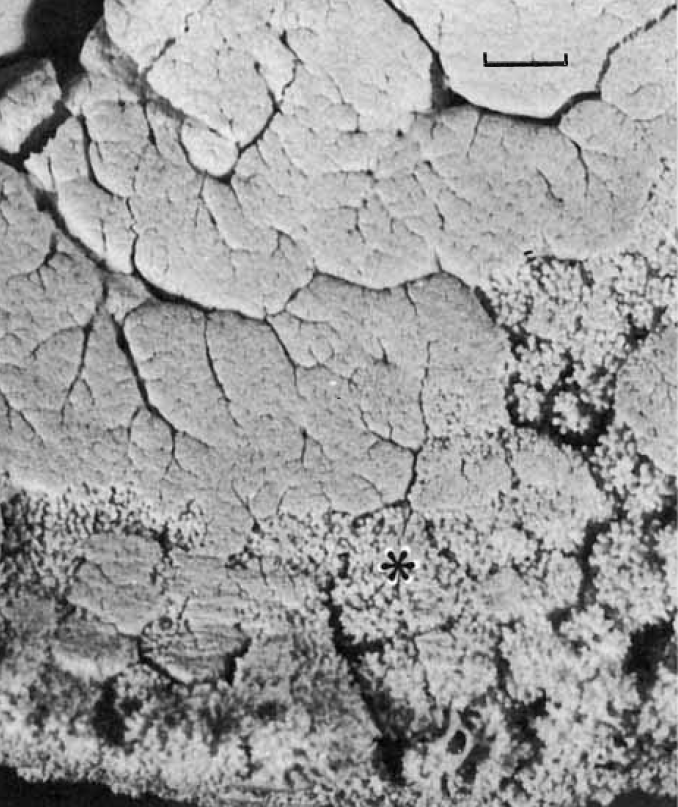
\includegraphics[width=0.35\textwidth,height=2in]{figures/images/upperlobe_haefeli1988.png}}                
  \subfloat[]{\label{fig:honey}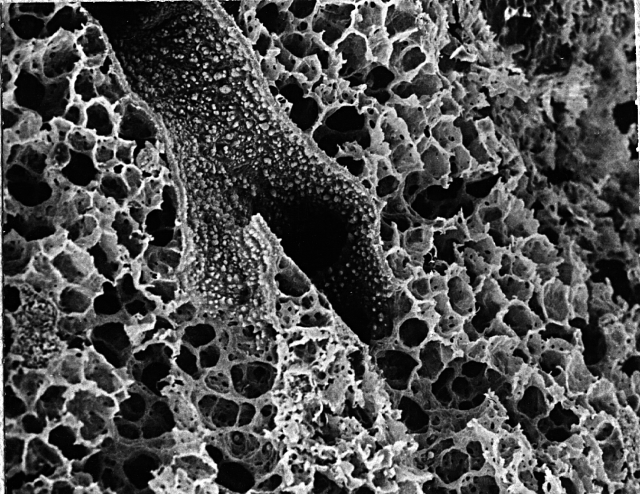
\includegraphics[width=0.35\textwidth,height=2in]{figures/images/TB_to_aveolarduct_BerkeleyLungLabtour.png}}\\
  \subfloat[]{\label{fig:pores}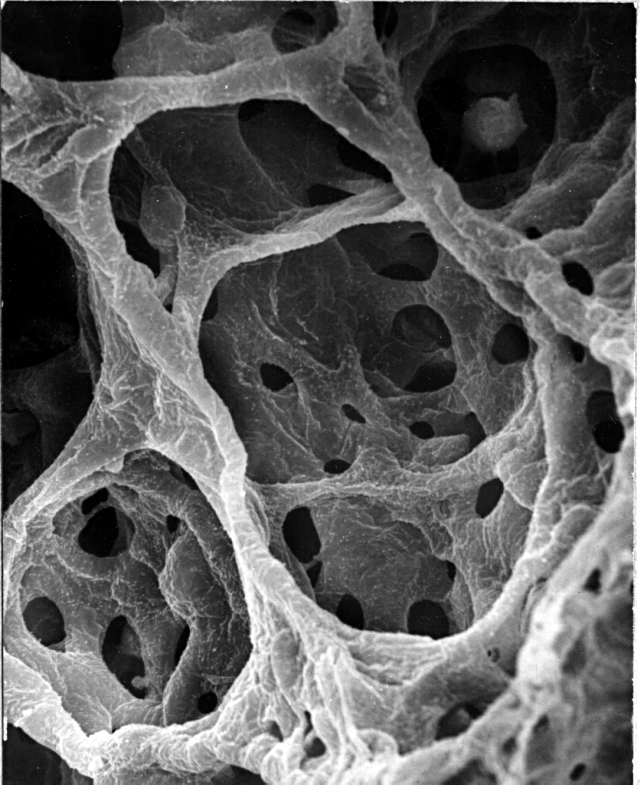
\includegraphics[width=0.35\textwidth,height=2in]{figures/images/aveolarPores_BerkeleyLungLabLungtour.png}}
\subfloat[]{\label{fig:acini}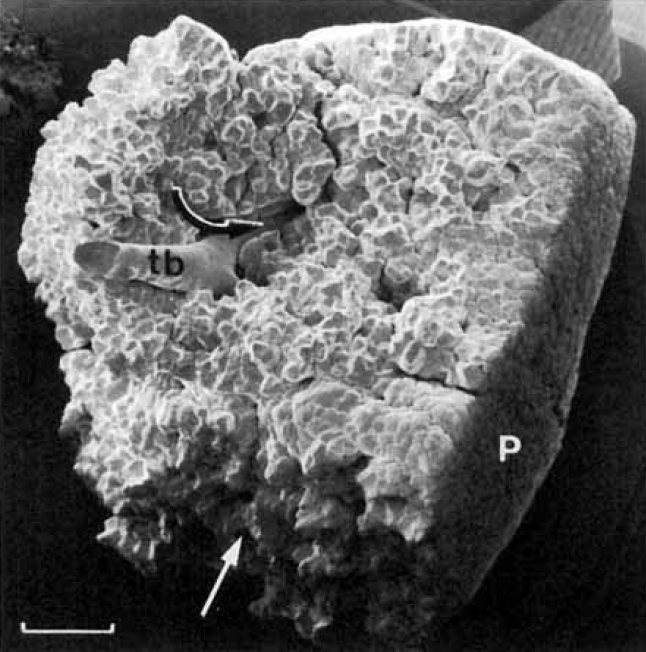
\includegraphics[width=0.35\textwidth,height=2in]{figures/images/acinus_HAEFELI-BLEUER1988.png}}
\caption{ (a) Portions of silicone rubber casts of upper lobes
of human lungs; asterisk marks incompletely filled regions. The outline of individual unfilled acinar units can also be seen. Scale marker, $5\;\mbox{mm}$. (b) Transition from terminal bronchiole to alveolar duct, from conducting airway to oxygen transfer area, diameter of terminal bronchiole is $0.5 \;\mbox{mm}$. (c) A few alveoli in an alveolar duct. The dark round openings are pores between alveoli. The alveolar wall is quite thin and contains a network of capillaries. The average diameter of one alveoli is $0.2\;\mbox{mm}$. (d) Scanning electron micrograph of complete acinus with transitional bronchiole
(tb) and surface abutting on pleura (P). Note the irregular surface where alveolar sacs of adjacent acini interdigitate (straight arrow). Scale marker, 1 mm. Images are reproduced from \cite{lunglab}.
 }
  \end{center}
   \label{fig:acinar_units}
\end{figure}
%
\begin{table}[h]
\begin{center}
\scalebox{0.76}{
\begin{tabular}{|l|c|c|c|c|c|c|}
\hline
Generation & Diameter & Length  & Flow rate 10L/min & Re & Flow rate 100L/min & Re \\
           & cm            & cm         &Velocity (m/s) &  & Velocity (m/s) & \\

\hline 
Trachea & 1.80 & 12.0 & 65.8 & 775 & 658 & 7750  \\
1 & 1.22 & 4.76 & 71.6 & 573 & 716 & 5730\\
5 & 0.35 & 1.07 & 53.6 & 123 & 536 & 1230\\
10 & 0.13 & 0.46 & 12.55 & 10.6 & 125 & 106\\
15 & 0.066 & 0.20 & 1.48 & 0.63 & 14.8 & 6.30\\
20 & 0.045 & 0.083 & 0.10 & 0.031 & 1.00 & 0.31\\

\hline
\end{tabular}
}
\end{center}
\caption{Shows dimensions, velocity and the corresponding Reynolds number for different sections of the airway tree during slow and rapid breathing. 
%Terminal bronchioles appear at around generation 15-16 which are then followed by respiratory bronchioles, the first generation to have alveoli. 
These values have been taken from \cite{pedley1970prediction}. }
\label{table:tree}
\end{table}
%
\begin{figure}[H]
  \centering
{\label{fig:mouse}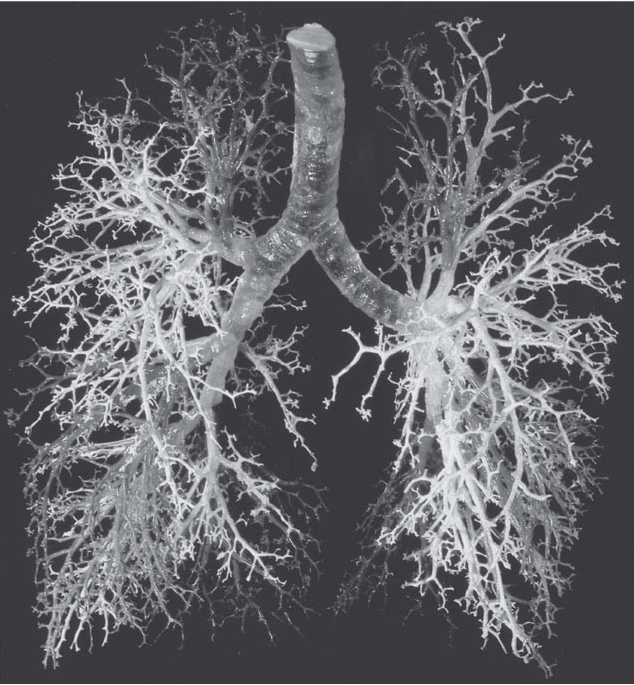
\includegraphics[width=0.5\textwidth]{figures/images/lung_west.pdf}}                
  \label{fig:acinar_units}
\caption{A rubber cast of the conducting of a human lung. The image is reproduced from \cite{west2008respiratory}.}
\label{fig:rubber_tree}
\end{figure}

%\subsubsection{Lung parenchyma} 
 Lung parenchyma refers to the portion of the lung made up of the small air chambers (alveoli) participating in gas exchange. The alveoli are made up of collagen, elastin fibers and membranous structures containing the capillary network, see Figure \ref{fig:pores}. Alveoli are arranged in sponge like structures and fill the entire volume of the lungs surrounding the conducting passages. Figure \ref{fig:sponge} shows a rubber cast of lung parenchyma, the dark lines outline the branching structure of the airways.
%The interior design of lung parenchyma is determined by the branching of the conducting airways. 
The right and left lung are partitioned into three and two lobes, respectively. Lung segments of conic shape are then the first subdivision of these lobes. These structures are bounded by connective tissue such that surgical separation is often possible. In the right lung, there are usually ten segments whereas only nine can be found in the left lung. Within the segments, the bronchi branch about six to twelve times. The terminal bronchioles which appear after roughly $15-16$ branching generations then finally feed into approximately $30,000$ so-called acini, see Figure \ref{fig:acini}. These acini represent the largest lung units of which all airways are alveolated and thus participate in gas exchange \cite{WeichertThesis}.
%
%
\begin{comment}
\subsection{Collateral ventilation.} 
Need to get a copy of the following paper:
``Collateral ventilation.
Menkes H, Traystman R, Terry P.
Abstract: Ventilation may bypass obstructed airways through collateral channels, including interalveolar pores of Kohn, bronchiole-alveolar communications of Lambert, and interbronchiolar pathways of Martin. Resistance through these channels, like resistance through small airways, increases with decreasing lung volume and with hypocapnia. But whereas the distention of collateral channels and small airways by a variety of factors is similar, the efficiency of ventilation through collateral channels is less than the efficiency through airways. Gas inspired through collateral channels is contaminated with alveolar gas from surrounding lung so that the dead space for collateral ventilation is increased. When one part of the lung ventilates out of phase with the surrounding lung, pulmonary interdependence promotes more homogeneous ventilation. In the presence of airways obstruction, interdependence may be a primary factor governing the rate of collateral ventilation. In man, collateral ventilation is unimportant in normal lungs. However, with disease, it may be critical in producing or compensating for abnormalities. For example, the long time constant for collateral ventilation in the middle lobe may be responsible for atelectasis, which results in the middle lobe syndrome. On the other hand, the short time constant for collateral ventilation in emphysema may be essential for the distribution of ventilation beyond obstructed airways.''

Also need to get:
``Collateral Ventilation and Gas Exchange during Airway Occlusion in the Normal Human Lung
Nicholas W. Morrell, C. Michael Roberts, Tony Biggs, and W. Anthony Seed''
\end{comment}
\begin{comment}

\begin{table}[H]
\begin{center}
\scalebox{0.7}{
\begin{tabular}{ l c c c c c}
\hline Parameter &  Description & Value& Reference  \\
\hline
$\rho^{s}$ & Density of alveolar tissue & ${1065\;\mbox{kg}}\,\mbox{m}^{-3}$ & \cite{hogg1969regional} \\
$\rho^{s}$ & Density of the alveolar wall & ${1000\;\mbox{kg}}\,\mbox{m}^{-3}$ & \cite{lande2006analysis}\\
$\rho^{f}$ & Density of of air at 27C$^\circ$ & ${1.18 \;\mbox{kg}}\,\mbox{m}^{-3}$ & Wiki \\
$\phi_{0}$ & Estimated reference porosity in the lung & $0.93$ & \cite{WeichertThesis} \\
$\mu^{f}$ & Viscosity for air at 27C$^\circ$ & $1.86 \times 10^{-5} \; \mbox{kg}\,\mbox{m}^{-1}\,\mbox{s}^{-1}$ & Wiki \\
$\bb{\kappa} $ &Permeability of the porous media (rough approximation) & $10^{-10}-10^{-12} \; \mbox{m}^{2}$ & \cite{owen2001mechanics},\cite{lande2006analysis}\\
$p $ &Mean airway pressure
 for high-frequency oscillation & $2000 \; \mbox{kg}\,\mbox{m}^{-1}\,\mbox{s}^{-2}$ & \cite{owen2001mechanics} \\
 $\hat{v} $ & Poisson ratio of porous lung at airway pressure $2000\,\mbox{Pas}$& $0.3$ & \cite{owen2001mechanics} \\
 
  $E $ & Young's modulus of lung tissue at airway pressure $2000\,\mbox{Pas}$& $8000$ $\mbox{kg}\,\mbox{m}^{-1}\,\mbox{s}^{-2}$  & \cite{owen2001mechanics} \\
  
  $\bb{u}^{s} $ & Tissue displacement near the diaphragm assuming sinusoidal motion & $0.05$ $\mbox{m}$  & \cite{gorman2002diaphragm} \\

  $\bb{a}^{s} $ & Tissue acceleration near the diaphragm assuming sinusoidal motion & $0.02$ $\mbox{m}\,\mbox{s}^{-2}$  & calculated \\

\hline
\end{tabular}
}
\end{center}
\caption{A collection of various parameters and typical values associated with lung parenchyma.} \label{tab:summary_equations}
\label{tab:parameters}
\end{table}
\end{comment}
%

%\section{Literature review}

%\input{/users/lorenzb/Dphil/poroelasticity_papers/coupling_paper/contents/literature}

\section{Computational lung models}
\label{section:review_models}
%
There exist a large number of computational ventilation and deformation models for the lung. Some models are designed to model particular phenomena whilst others are more general. They also range in spatial complexity from 0D compartment type models to 3D models which are able to incorporate `patient-specific' geometries extracted from CT images. In this review, we will focus on models that couple ventilation with tissue deformation and can be used as patient-specific models. A review of popular compartment based lung models can be found in \citet{bates2009lung}. 
%
One study that couples ventilation and tissue deformation using a one way coupling approach and then applies the model to a full 3D geometry is described in \citet{tawhai2010image}. Here a mechanics model for elastic deformation of compressible lung tissue is used to provide flow and pressure boundary conditions for an embedded airway model which makes the resultant ventilation distribution dependent on the tissue deformation due to gravity. In \citet{Swan2012}, air flow is simulated in patient specific conducting airways which are coupled to geometrically simplified terminal acinar units with varying volume dependent compliance. The fluid flow in the airways is approximated by Poiseuille flow with an added correction term for airway bifurcations. The end terminal acinar units are able to expand but are assumed to be independent of neighbouring acinar units. This does not allow for feedback from neighbouring acini that are infact tightly connected by a matrix of fibers, collagen and capillaries. 
%This model confirms experimental evidence that in the healthy lungs tissue compliance has a far greater effect than airway resistance on the spatial distribution of ventilation, and hence a realistic description of tissue deformation is essential in models of ventilation. 
Other sophisticated flow models of the whole airway tree, also exist \citep{yin2013multiscale,ismail2013coupled}. These models solve the full 3D Navier-Stokes equations in the upper airways, segmented from CT images, to capture high Reynolds number effects. The 3D fluid model is then coupled to a 0D laminar flow model of the lower airways. %None of these models incorporate the feedback of tissue deformation on ventilation and vice versa, and only loosely couple tissue deformation to ventilation.  


\section{Poroelastic models for lung parenchyma and other biological tissue}
%\label{section:poroelastic_review}
Some early work on a mechanical model of lung parenchyma as a poroelastic medium has already been proposed in \citet{kowalczyk1993mechanical}. This work developed a similar poroelastic model to the one we propose, however it has only been applied to a very simple 2D geometry. Also in \citet{owen2001mechanics} homogenisation theory has been used to derive macroscopic poroelastic equations for average air flows and tissue displacements in lung parenchyma during high frequency ventilation. The resulting model is a one dimensional system of equations that is used to investigate the effect of high-frequency ventilation on strain in the parenchymal tissue. The use of a poroelastic model has also been applied to modelling other biological tissues. For example modelling protein based hydrogels embedded with cells \citep{galie2011linear}, perfusion of blood flow in the beating myocardium \citep{chapelle2010poroelastic,cookson2011novel}, the modelling of brain oedema (swelling) \citep{li2010three} and hydrocephalus \citep{wirth2006axisymmetric}. Another application is the modelling of interstitial fluid and tissue in articular cartilage and intervertebral discs \citep{mow1980biphasic,holmes1990nonlinear,galbusera2011comparison}.




\begin{comment}
%One study presented a framework for coupling models of ventilation and tissue deformation \cite{tawhai2006imaging}. First, changes in geometry of the lung mesh are determined and used to compute flow through an airway model. Pressures are then interpolated throughout the lung mesh to provide hydrostatic pressures that act as input loads for the mechanics model, which is then solved to predict shape change. These deformations are used to compute local volume changes which feed back as inputs to the flow-pressure problem and the system is solved iteratively. In these models tissue deformation is not directly dependent on ventilation, however an integrated model of ventilation and tissue mechanics model will be particularly important for understanding respiratory diseases since nearly all pulmonary diseases lead to some abnormality of lung tissue mechanics  \cite{suki2011lung}. For example, Chronic Obstructive Pulmonary Disease (COPD) encompasses emphysema (destruction of alveolar tissue) and chronic 
bronchitis which can cause severe bronchoconstriction and atelectasis (air trapping), both of which can significantly alter tissue properties. If the tissue mechanics are affected so too will the ventilation and vice versa emphasising the importance of a model that fully couples the tissue mechanics and ventilation in the lung. 

%There has been one study that presents a framework for coupling models of ventilation and tissue deformation \cite{tawhai2006imaging}. First, changes in geometry of the lung mesh are determined and used to compute flow through an airway model. Pressures are then interpolated throughout the lung mesh to provide hydrostatic pressures that act as input loads for the mechanics model, which is then solved to predict shape change. These deformations are used to compute local volume changes which feed back as inputs to the flow-pressure problem and the system is solved iteratively.

 %Although it is assumed that lung tissue is a continuum with uniform material properties, simulations of tissue deformation in a realistic geometry can give rise to a considerable degree of heterogeneity. 
%Including this model of tissue deformation in a ventilation model clearly predicts more physiologically consistent ventilation distributions than simply assuming that tissue compliance is constant or proportional to lung height. Therefore we conclude  that it is an essential feature in functional computational models of ventilation which aim to describe ventilation and perfusion matching or changes in ventilation distribution with disease.
%Another model that incorporates subject-specific anatomical geometry and approximates the airways by Poiseuille flow with an added correction term for airway bifurcations is presented in \cite{HedgesThesis}, here the aim is to predict forced expiration (FEV1) values. 

\end{comment}



 
%The model confirms experimental evidence that in the healthy lungs tissue
%compliance has a far greater effect than airway resistance on the spatial distribution of ventilation, and hence a realistic description of tissue deformation is essential in models of ventilation.
%Although it is assumed here that lung tissue is a continuum with uniform material properties, simulations of tissue deformation in a curvilinear geometry can give rise to a considerable degree of heterogeneity. Including this model of tissue deformation in a ventilation model clearly predicts more physiologically consistent ventilation distributions than simply assuming that tissue compliance is constant or proportional to lung height. Therefore we conclude  that it is an essential feature in functional computational models of ventilation which aim to describe ventilation and perfusion matching or changes in ventilation distribution with disease.''  \cite{SwanThesis}

 %However in this model, tissue deformation is not directly dependent on ventilation.


%Due to the often high Reynolds numbers in the upper airways, 3D fluid flow models have been used to model this sections of the airway tree. Clearly approximating the entire airway tree using 3D fluid flow remains intractable due to constraints on imaging resolution and computational power. Therefore smaller airways still need to be generated using a volume-filling branching algorithm \cite{tawhai2004ct} and then approximated by simpler 1D flow equations. The coupling of a 3D flow model to a 1D flow model for a complete airway tree has already been done in \cite{lin2009multiscale} and is achieved through mass conservation. i.e. the flow rates at the exit faces of the 3-D airway model can be determined by summing the flow rates at the terminal bronchioles using the connectivity information between the 3-D airway exit faces and the associated downstream 1-D airway branches. However this summing of flow rates is unable to account for any changes in resistances in the airway tree which might have been introduced 
%due to disease, for example bronchoconstriction or the collapsing of airways which is common in many types of COPD. There has also been sophisticated work on 3D to 1D fluid flow coupling for modelling blood flow with compliant vessels in the cardiovascular system \cite{formaggia2001coupling} and cerebral vasculature \cite{passerini20093d}.



%\input{/users/lorenzb/Dphil/poroelasticity_papers/large_deformation/contents/review}
\section{Finite element methods for poroelasticity}
The method that we use for spatially discretising our equations in this work is the finite element method (FEM) for obtaining approximations to the solution of partial differential equations.

After many decades of research there remain numerous challenges associated with the numerical solution of the poroelastic equations. When using the finite element method the main challenge is to ensure stability and convergence of the method and prevent numerical instabilities that often manifest themselves in the form of spurious oscillations in the pressure. It has been suggested that this problem is caused by the saddle point structure in the coupled equations resulting in a violation of the famous Ladyzhenskaya-Babuska-Brezzi (LBB) condition \citep{haga2012causes}, highlighting the need for a stable combination of mixed finite elements. Another numerical challenge in practical 3D applications is the algebraic system arising from the finite element discretisation. This can lead to a very large matrix system that has many unknowns and is severely ill-conditioned, making it difficult to solve using standard iterative solvers. Therefore low-order finite element methods that allow for efficient preconditioning are preferred \citep{white2011block,ferronato2010fully}.

\subsection{Linear three-field discretisations}
The poroelastic equations are often solved in a reduced displacement and pressure formulation, from which the fluid flux can then be recovered \citep{murad1994stability,white2008stabilized}. \citet{murad1994stability} have analysed the stability and convergence of this reduced displacement pressure $(\boldsymbol{u}/ p)$ formulation and were able to show error bounds for inf-sup stable combinations of finite element spaces (e.g. Taylor-Hood elements). In this paper we will keep the fluid flux variable resulting in a three-field, displacement, fluid flux, and pressure formulation. Keeping the fluid flux as a primary variable has the following advantages:
\begin{enumerate}[label=\roman*]
 \item It avoids the calculation of the fluid flux in post-processing. 
\item Physically meaningful boundary conditions can be applied at the interface when modelling the interaction between a fluid and a poroelastic structure \citep{badia2009coupling}.
 \item It allows for greater accuracy in the fluid velocity field. This can be of interest whenever a consolidation model is coupled with an advection diffusion equation, e.g. to account for thermal effects, contaminant transport or the transport of nutrients or drugs within a porous tissue \citep{khaled2003role}.
 \item It allows for an easy extension of the fluid model from a Darcy to a Brinkman flow model, for which there are numerous applications in modelling biological tissues \citep{khaled2003role}.
 \item It reduces the order of the spatial derivative of the pressure, allowing for a discontinuous pressure approximation without any additional penalty terms.
\end{enumerate}

\citet{phillips2007coupling,phillips2007couplingtwo}, have proven error estimates when solving the three-field formulation problem using continuous piecewise linear approximations for displacements and mixed low-order Raviart Thomas elements for the fluid flux and pressure variables. However this method was found to be susceptible to spurious pressure oscillations \citep[see,][]{phillips2009overcoming}. To overcome these pressure oscillations, \citet{li2012discontinuous} analysed a discontinuous three-field method, and \citet{yi2013coupling} analysed a nonconforming three-field method.
%In \citet{li2012discontinuous}, a discontinuous method and in \citet{yi2013coupling} a nonconforming three-field method is analysed. These papers were motivated by the need for a method that is able to overcome pressure oscillations \citep[see,][]{phillips2009overcoming} experienced by the method in \citet{phillips2007coupling,phillips2007couplingtwo}. 
In addition to these monolithic approaches there has been considerable work on operating splitting (iterative) approaches for solving the poroelastic equations \citep{wheeler2007iteratively,feng2010fully,kim2011stability}. Although these methods are often able to take advantage of existing elasticity and fluid finite element software, and result in solving a smaller system of equations, these schemes are often only conditionally stable. To ensure that the method is unconditionally stable, monolithic approaches are often preferred. The method proposed in this work is monolithic, and will therefore retain the advantage of being unconditionally stable .

%\subsection{Stability of Darcy-Stokes formulation}
%Numerous stabilization techniques for finite element methods have already been proposed in order to satisfy the LBB condition, most extensively for the model equations of Stokes and Darcy flow, which despite their simplicity retain all the difficulties of a saddle point problem. This will be discussed again in more detail in section \ref{sec:mixed}. Another good introduction on stabilization techniques for the Stokes problem can be found in chapter 5 of \citet{elman2005finite}. For a comparison of low-order stabilization techniques for the Darcy problem we refer to \citet{bochev2006computational}. Most stabilized methods lead to a modified variational formulation in which an additional term is added to the mass balance equation, modifying the incompressibility constraint
%in such a way that stability of the mixed formulation is increased,
%while still maintaining optimal convergence of the method. These stabilization techniques are of great interest to us since solving the three-field poroelasticity problem is essentially equivalent to coupling the Stokes equations (elasticity of the porous mixture) with the Darcy equations (fluid flow through pores), with a modified incompressibility constraint that combines the divergence of the displacement velocity and the fluid flux. 







%After many decades of research there remain numerous challenges associated with the numerical solution of the poroelastic equations valid in small and large deformations. When using the finite element method the main challenge is to ensure stability and convergence of the method and prevent numerical instabilities that often manifest themselves in the form of oscillations in the pressure. It has been suggested that this problem is caused by the saddle point structure in the coupled equations resulting in a violation of the famous Ladyzhenskaya-Babuska-Brezzi (LBB) condition \citep{haga2012causes}, highlighting the need for a stable combination of mixed finite elements. Another numerical challenge in practical 3D applications is the algebraic system arising from the finite element discretization. These theoretical stability issues have already been studied for some linear (small deformation) poroelasticity formulations \citep{murad1994stability,haga2012causes} and numerous remedies have been proposed \citep{phillips2007coupling,phillips2007couplingtwo,li2012discontinuous,yi2013coupling,berger2014stabilized}.
\subsection{Methods valid in large deformations}


We will now give a brief overview of different approaches for solving the poroelastic equations valid in large deformations. There has been some work on operating splitting (iterative) approaches where the poroelastic equations are separated into a fluid problem and deformation problem \citep{chapelle2010poroelastic}. Again, this approach is only conditionally stable. Some notable quasi-static incompressible large deformation monolithic approaches include a mixed-penalty formulation, and a mixed solid velocity-pressure formulation, both outlined in \citep{almeida1998finite}, the solid velocity-pressure formulation is similar to the commonly used reduced $(\boldsymbol{u}/p)$ formulation \citep{ateshian2010finite}. These two-field $(\boldsymbol{u}/p)$ formulations require a stable mixed element pair such as the popular Taylor-Hood element to satisfy the LBB inf-sup stability requirement. To reduce the number of unknowns, and allow for an equal-order, piecewise linear approximation, a stabilized reduced $(\boldsymbol{u}/ p)$ formulation has been proposed in \citep{white2008stabilized}. This method introduces a stabilization term to the mass conservation equation to overcome the spurious pressure oscillations. The key difficulty, however, that this stabilized element cannot escape is that jumps in material coefficients may introduce large solution gradients across the
interface, requiring severe mesh refinement. This is because a continuous pressure element is used, which is unable to reliably capture jumps in the pressure solution \citep{white2008stabilized}. In \citep{levenston1998variationally} a three-field (displacement, fluid flux, pressure) formulation has been outlined, however this method uses a low-order mixed finite element approximation without any stabilization and therefore is not inf-sup stable.





 


%\input{/users/lorenzb/Dphil/poroelasticity_papers/ima_submission/introduction_jcam}

\chapter{Poroelasticity theory}
\input{/users/lorenzb/Dphil/poroelasticity_papers/large_deformation/contents/intro_theory}
\section{Kinematics}
\input{/users/lorenzb/Dphil/poroelasticity_papers/large_deformation/contents/continuum_mechanics_theory}

%\section{Mixture theory}
\input{/users/lorenzb/Dphil/poroelasticity_papers/large_deformation/contents/mixture_theory}


\section{Linear poroelasticity}
\label{sec:themodel}
To allow us to perform rigorous analysis of the proposed finite element scheme presented in Chapter \ref{chap:linear_poro}, we will now assume small deformations to yield a linear model of poroelasticity. This model is often referred to as the `Biot model' in the geomechanics community and contains some additional terms. We will introduce the full Biot model here for use with a 2D cantilever bracket problem later tested in section \ref{section:overcoming}, and to highlight that any subsequent theory developed in later chapters can be extended to the full Biot model. The governing equations of the Biot model, with displacement $\dispcont$, fluid flux $\fluxcont$, and pressure $\pcont$ as primary variables are summarized below:  
\begin{subequations}
\begin{align}
\label{eqn:strong_mixture_momentum}
- \nabla \cdot \mathbf{\sigma}  =\mathbf{f} \;\;\; \mbox{in}\; \Omega \times (0,T),\\
{\perm^{-1}\mathbf{z}} + \nabla p =  \mathbf{b} \;\;\; \mbox{in}\; \Omega\times (0,T), \\
\nabla \cdot \mathbf{z} + \pderiv{}{t}(\alpha\nabla \cdot \mathbf{u} + c_{0} p )  = g   \;\;\; \mbox{in}\; \Omega \times (0,T),
\\
\mathbf{u} =\mathbf{u}_{D}   \;\;\; \mbox{on}\; \Gamma_{D} \times (0,T),
\\
\mathbf{\sigma}\mathbf{n} = \mathbf{t}_{N}   \;\;\; \mbox{on}\; \Gamma_{N} \times (0,T),
\\
p = p_{D}   \;\;\; \mbox{on}\; \Gamma_{P} \times (0,T),
\\
\mathbf{z}\cdot \mathbf{n} = {q_{D}}   \;\;\; \mbox{on}\; \Gamma_{F} \times (0,T),
\\
\mathbf{u}(0,\cdot) = \mathbf{u}^{0},  \;\;\; p(0) = p^{0}, \;\;\; \mbox{in}\; \Omega.
\end{align}
\label{eqn:strong_cont_system_biot}
\end{subequations}
Here $\mathbf{\sigma}$ is the total stress tensor given by $\mathbf{\sigma}=\lambda \mbox{tr}(\mathbf{\epsilon}(\dispcont))\identity + 2\mu_{s}\mathbf{\epsilon}(\dispcont)-\alpha p\mathbf{I}$, with the linear strain tensor defined as $\mathbf{\epsilon}(\dispcont)=\frac{1}{2}\left(\nabla \dispcont + \left( \nabla \dispcont \right)^{T} \right)$, $g$ is the fluid source term, $\mathbf{f}$ is the body force on the mixture, and $\mathbf{b}$ is the body force on the fluid.  Here $\Omega$ is a bounded domain in $\mathbb{R}^{2}$ or $\mathbb{R}^{3}$, and for the purpose of defining boundary conditions, $\partial\Omega=\Gamma_D+\Gamma_N$ for displacement and stress boundary conditions and  $\partial\Omega=\Gamma_P+\Gamma_F$ for pressure and flux boundary conditions, with outward pointing unit normal $\mathbf{n}$. The parameters along with a description are given in Table \ref{tab:parameters}.
\begin{table}[H]
\begin{center}
\scalebox{0.9}{
\begin{tabular}{ l c c }
\hline
\bf Parameter &    \\
\hline
Lam\'{e}'s first parameter &  $\lambda$,  \\
Lam\'{e}'s second parameter (shear modulus)  &  $\mu_{s}$,  \\
Dynamic permeability tensor &  $\perm$,  \\
%Solid skeleton density &  $\rho_s$  \\
%Fluid density &  $\rho_f$  \\
Biot-Willis constant &  $\alpha$,  \\
Constrained specific storage coefficient &  $c_{0}$.
\end{tabular}
}
\end{center}
\caption{Poroelasticity parameters.} 
\label{tab:parameters}
\end{table}
\noindent A derivation and more detailed explanation of these equations can be found in \citet{phillips2007coupling} and \citet{showalter2000diffusion}. In this work we will mainly consider a simplification of the full Biot model (\ref{eqn:strong_cont_system_biot}), by setting $\alpha=1$ and $c_{0}=0$. This yields a fully incompressible poroelastic model that retains all the numerical difficulties associated with approximating the original system of equations (\ref{eqn:strong_cont_system_biot}), see Remark \ref{remark:extension}. The linear fully saturated and incompressible poroelastic model is given by: 
\begin{subequations}
\begin{align}
\label{eqn:strong_mixture_momentum_simple}
-(\lambda+\mu_{s}) \nabla (\nabla\cdot\mathbf{u})-\mu_{s} \nabla^{2} \mathbf{u} + \nabla p = \mathbf{f} \;\;\; \mbox{in}\; \Omega\times (0,T),\\
{\perm^{-1}\mathbf{z}} + \nabla p =  \mathbf{b} \;\;\; \mbox{in}\; \Omega\times (0,T),\\
\nabla \cdot (\mathbf{u}_{t} + \mathbf{z} )  = g   \;\;\; \mbox{in}\; \Omega\times (0,T),
\\
\mathbf{u} =\mathbf{u}_{D}   \;\;\; \mbox{on}\; \Gamma_{D}\times (0,T),
\\
\mathbf{\sigma}\mathbf{n} = \mathbf{t}_{N}   \;\;\; \mbox{on}\; \Gamma_{N}\times (0,T),
\\
p = p_{D}   \;\;\; \mbox{on}\; \Gamma_{P}\times (0,T),
\\
\mathbf{z} \cdot \mathbf{n} = {q_{D}}   \;\;\; \mbox{on}\; \Gamma_{F}\times (0,T),
\\
\mathbf{u}(0,\cdot) = \mathbf{u}^{0}  \;\;\;  \mbox{in}\;\Omega.
\end{align}
\label{eqn:linear_simple_system}
\end{subequations}

\noindent This model is the small deformation version of the simplified and reformulated large deformation poroelasticity model (\ref{eqn:simple_mixture_model}), and will be the small deformation model considered from here onwards.


\begin{remark}
The extension of the theoretical results presented in Chapter \ref{chap:linear_poro} from (\ref{eqn:linear_simple_system}) to the full Biot equations (\ref{eqn:strong_cont_system_biot}), with $\alpha \in \mathbb{R}_{> 0} \text{ and } c_{0}\in \mathbb{R}_{> 0}$ is straightforward. In the analysis in Chapter \ref{chap:linear_poro}, the constant $\alpha$ would just get absorbed by a general constant $C$. When $c_{0}>0$, an additional pressure term is introduced into the mass conservation equation. Since this term is coercive, it only improves the stability of the system.
\label{remark:extension}
\end{remark}







%% FEM intro
\chapter{Finite element method}

\section{Introduction}
%Miguel
A large proportion of the mathematical models in science and engineering take the
form of differential equations. Only in the simplest cases, or under strong assumptions,
is it possible to find exact analytical solutions to the equations in the model.
%Often, one has to rely on numerical techniques for finding approximate solutions
%for particular parameter sets using computers. 
%The finite element method is a general
%technique for the numerical solution of differential equations. 
%
%The method was introduced by engineers in the late 1950's and early 1960's for the numerical
%solution of PDEs in structural engineering. When the mathematical study
%of the finite element method started in the mid 1960's it soon became clear that in
%fact the method is a general technique for numerical solution of partial differential
%equations with roots in the variational methods in mathematics introduced at the
%beginning of the 20th century.
%
%
%
%
%Lyia
Numerical methods are an established means of solving differential equations that are
of practical interest in a variety of applied problems. Finite difference, finite volume
and finite element methods are the most widely used types of such methods. Their
basic idea is replacing the infinite-dimensional problem by a finite-dimensional
approximation, which is, generally speaking, easier to compute.
%
%The main idea of finite difference methods is to approximate the derivatives appearing
%n the equations with finite differences at a set of discrete points in the domain
%of interest. Their advantages include relative simplicity of derivation and implementation.
%However, finite difference methods are best suited for simple domain shapes
%and regular meshes, while using them for problems on complex geometries requires
%non-standard treatment even for standard differential equations. For an introduction
%to finite differences in partial differential equations we refer to [90, 116, 114].
%Finite volume methods [87, 121] rely on the application of the divergence theorem
%within small subdomains of the original domain – finite volumes – and approximating
%fluxes through volume boundaries. These methods are traditionally used in the
%field of computational fluid dynamics due to their conservative properties, although
%9
%formulating problems on complex geometries is again far from trivial.
Finite element methods are based on weakening the restrictions on the solution
space in the continuous setting, and searching for the approximate solution in the
subspace which spans basis functions supported on small regions inside the domain.
These methods are well-suited to solving problems on complex domains, and are
therefore widely used in practical applications.
In this work we consider only finite element methods (FEMs) for solving partial
differential equations.
This chapter comprises an overview of several theoretical and practical aspects of classical FEMs. The theory and notation presented here are essential in developing
the techniques that form the core of this thesis. Most of the work presented in this chapter is based on work already presented in \citet{arthursthesis,asnerthesis,bernabeusthesis,brenner2008mathematical,f1991mixed}.


%
%Chris
%The method that we use for spatially discretising our equations in this work is the finite
%element method (FEM) for obtaining approximations to the solution of partial differential
%equations. It was introduced in its present form in 1942 by Richard L. Courant as an
%appendix to his paper on variational methods [75], although it does not then appear in
%the literature again for another sixteen years [76]. It was further developed by engineers
%during the late 1950s and early 1960s as a method of solving equations in structural engineering
%[77], and has since developed into a general tool for the numerical approximation
%of solutions to PDEs.
\section{Norms and spaces}
Let $\Omega$ be a bounded domain in $\mathbb{R}^{2}$ or $\mathbb{R}^{3}$, and $\partial\Omega$ be the associated boundary. The space of square integrable functions is then given by
\begin{equation*}
L^{2}(\Omega)  = \left\lbrace  u : \int_{\Omega} |u(x)|^{2} \mbox{d}x < \infty \right\rbrace,
\end{equation*}
with norm
\begin{equation*}
\ltwonorm{u}  = \left\lbrace \int_{\Omega} |u(x)|^{2} \mbox{d}x  \right\rbrace^{1/2}.
\end{equation*}
This space is equipped with the inner product
\begin{equation*}
(u,v)  :=  \int_{\Omega} u(x)v(x) \mbox{d}x,
\end{equation*}
such that $\ltwonorm{u}=(u,v)^{1/2}$. Throughout this thesis we shall frequently refer to the Sobolev spaces
$H^{1}(\Omega)$ and $H^{2}(\Omega)$. The definitions of these are as follows:
%
\begin{equation*}
H^{1}(\Omega)  = \left\lbrace  u  \in L^{2}(\Omega): \frac{\partial u }{\partial x_{j}} \in L_{2}(\Omega) , \; j=1,\ldots ,n, \right\rbrace,
\end{equation*}
\begin{equation*}
H^{2}(\Omega)  = \left\lbrace  u  \in L^{2}(\Omega): \frac{\partial u }{\partial x_{j}} \in L_{2}(\Omega) , \; j=1,\ldots ,n, \;  \frac{\partial^{2} u }{\partial x_{i} \partial x_{j}} \in L_{2}(\Omega), \; i,j=1,\ldots ,n \right\rbrace.
\end{equation*}
The corresponding norms are defined as
\begin{equation*}
\honenorm{u}  = \left\lbrace \ltwonorm{u}^{2} + \sum_{j=1}^{n} \ltwonorm{\frac{\partial u }{\partial x_{j}}}   \right\rbrace^{1/2},
\end{equation*}
\begin{equation*}
\htwonorm{u}  = \left\lbrace \ltwonorm{u}^{2} + \sum_{j=1}^{n} \ltwonorm{\frac{\partial u }{\partial x_{j}}}  + \sum_{i,j=1}^{n} \ltwonorm{\frac{\partial^{2} u }{\partial x_{i} \partial x_{j}}}  \right\rbrace^{1/2}.
\end{equation*}
We also define the divergence space 
\begin{equation*}
H_{div}(\Omega)=\left\lbrace \boldsymbol{v}\in L^{2}(\Omega): \nabla \cdot \boldsymbol{v} \in L^{2}(\Omega) \right\rbrace.
\end{equation*}
The set of functions of $L^{2}(\partial \Omega)$ which are traces of functions of $H^{1}(\Omega)$ onto the boundary, constitutes a subspace of $L^{2}(\partial \Omega)$ denoted by $H^{1/2}(\partial \Omega)$. We will also briefly use linear and bounded functionals (dual spaces) of $H^{1},H^{1/2}$ and $H_{div}$, which will be denoted by $H^{-1},H^{-1/2}$ and $H_{div}^{-1}$, respectively. 

We define the following norms for continuous in time functions $u$ such that the norm $L^2(0,T; X)$ satisfies
\begin{equation*}
 || u ||_{L^2( X) }= \left( \int_0^T || u (s,\cdot) ||^2_X ~ds \right)^{1/2},
\end{equation*}
and the norm $L^{\infty}(0,T; X)$ satisfies
\begin{equation*}
 || u ||_{L^{\infty}(X) }= \sup\left\lbrace ||{u (s,\cdot)}||_{X} : s \in [0,T] \right\rbrace,
\end{equation*}
where $X$ is any given function space over $\Omega$. We partition $[0,T]$ into $N$ evenly spaced non-overlapping regions $(t_{n-1}, t_n]$, $n=1,2,\dots, N$. For any sufficiently smooth function $u(t,x)$ we define $u^n(x) = u(t_n,x)$. Let the discrete approximation for all time to be the piecewise constant in time functions $v(t,{\bf x})  := v^n({\bf x})$ for $t \in (t_{n-1}, t_n]$. For such piecewise constant in time functions, $v$, we define the norms
\begin{equation*}
 || v ||_{L^2( X) }= \left( \sum_{n=1}^N \Delta t   || v^n||^2_X \right)^{1/2},
\end{equation*}
and
\begin{equation*}
 || v ||_{L^{\infty}( X) }= \max\left\lbrace ||{v^n}||_{X}, n=1,2,...,N \right\rbrace.
\end{equation*}




\begin{comment}

Finally we define the following continuous time-dependent norms 
\begin{equation*}
   \doublenorm{v}_{L^{2}(L^{2})} = \left( \int_{0}^{T} \ltwonorm{v(\cdot,t_{n})}^{2} dt \right)^{1/2}            ,                                                                                                                                                                                                                                                                                                                                                                                                                                                                                                                                                                                                                                                                                                                                                                                                                                                                                                                                                                                                                                                                                         \end{equation*}
   \begin{equation*}
   \doublenorm{v}_{L^{\infty}(L^{2})} =  \sup\left\lbrace \ltwonorm{v(\cdot,t_{n})} : t_{n} \in [0,T] \right\rbrace,                                                                                                                                                                                                                                                                                                                                                                                                                                                                                                                                                                                                                                                                                                                                                                                                                                                                                                                                                                                                                                                                                                    \end{equation*}
and their discrete in time counterparts
\begin{equation*}
  \doublenorm{v}_{l^{2}(L^{2})} = \left( \sum_{n=0}^{N} \Delta t_{n} \ltwonorm{v(\cdot,t_{n})}^{2} \right)^{1/2}            ,                                                                                                                                                                                                                                                                                                                                                                                                                                                                                                                                                                                                                                                                                                                                                                                                                                                                                                                                                                                                                                                                                         \end{equation*}
   \begin{equation*}
  \doublenorm{v}_{l^{\infty}(L^{2})} =  \max\left\lbrace \ltwonorm{v(\cdot,t_{n})} : t_{n} \in [0,t_{1},t_{2},...,T] \right\rbrace.                                                                                                                                                                                                                                                                                                                                                                                                                                                                                                                                                                                                                                                                                                                                                                                                                                                                                                                                                                                                                                                                                           \end{equation*} Definitions for slightly different combinations of temporal and spatial norms such as $\doublenorm{v}_{H^{1}(L^{2})}$ are straightforward adaptations of the above. Additional shorthand notation will be introduced throughout the thesis as is needed.

\end{comment}




%Let $L^{2}(\Omega)  := \left\lbrace  u : \int_{\Omega} u^{2} < \infty %\right\rbrace$ be the usual space of square integrable functions with inner %product $(v,w)=  \int_{\Omega} v(x)w(x) \mbox{d}x $ and norm $\ltwonorm{v}= %(v,v)^{1/2}$. We further define $L_{0}^{2}=\lbrace \pconttest \in L^{2}(\Omega): %\int_{\Omega} \pconttest = 0  \rbrace$.  
%
%We also introduce the space of functions with derivatives $\partial^{{\alpha}}v \in L^{2}(\Omega)$ for $|{\alpha}| \leq m$, where $ {\alpha}=\left\lbrace \alpha_{1}, \alpha_{2} \right\rbrace$, $|{\alpha}|= \alpha_{1}+\alpha_{2}$, $\alpha_{i}$ non-negative integers, equipped with the inner product $(v,w)_{m}=  \int_{\Omega} \partial^{\alpha} v(x) \partial^{\alpha}w(x) \mbox{d}x $ and norm $\hmnorm{v}= (v,v)_{m}^{1/2}$. 
%
%
%
\section{Model problem}
It is instructive to begin at a simple level and proceed by incrementally adding to the
complexity of the equations we are discretising when explaining the use of the FEM, so
we begin by considering the classical heat equation: given $T>0$, for $t \in[0,T]$ find $u(t,x)$ such that
\begin{subequations}
\begin{align}
\label{eqn:heat_strong}
\frac{\partial u}{\partial t} - \nabla \cdot \nabla u = 0\;\;\; \mbox{in} \; \Omega_{t},\\
\boldsymbol{n} \cdot \nabla u = {g}_{N}   \;\;\; \mbox{on}\; \Gamma_{N},
\\
\label{eqn:heat_dirichlet}
 u = {g}_{D}   \;\;\; \mbox{on}\; \Gamma_{D},
\\
 u(0,x) = u^{0}(x)   \;\;\; \mbox{in}\; \Omega.
\end{align}
\label{eqn:laplace}
\end{subequations}
Here $\Omega$ is a bounded domain in $\mathbb{R}^{2}$ or $\mathbb{R}^{3}$, with boundary $\partial\Omega = \Gamma_{N}  \cup \Gamma_{D} $, that has an outward pointing unit normal $\boldsymbol{n}$. The initial condition is given by $u^{0}(x)$. In the case where ${g}_{N}= 0$, system (\ref{eqn:laplace}) can describe the evolution of heat in an
object with geometry described by $\Omega$, where we have perfect thermal insulation on $\Gamma_{N}$ and fixed temperature distributions given by the function ${g}_{D}$ defined on the boundary due to some part of the environment with fixed temperature contacting the object along $\Gamma_{D}$.

\subsection{Weak formulation}

The strong form of (\ref{eqn:laplace}) requires $u$ to be at least twice differentiable. To weaken the regularity restrictions we multiply equation (\ref{eqn:heat_strong}) by an arbitrary function $v$, called a test function, and integrate over $\Omega$: 
\begin{equation*}
\left( \frac{\partial u}{\partial t},v \right)  -\left(\nabla \cdot \nabla u,v \right) = 0.
\end{equation*}
Applying the divergence theorem, this equation can be rewritten:
\begin{multline*}
\left( \frac{\partial u}{\partial t},v \right)  -\left(\nabla u \cdot \normal ,v \right)_{\partial \Omega}+ \left(\nabla u,\nabla v \right)\\= \left( \frac{\partial u}{\partial t},v \right)  -\left(\nabla u \cdot \normal ,v \right)_{\Gamma D}-\left(g_{N} ,v \right)_{\Gamma N}+ \left(\nabla u,\nabla v \right)=0.
\end{multline*}
Here $\left(\cdot ,\cdot\right)_{\Gamma_{N}}$ and $\left(\cdot ,\cdot\right)_{\Gamma_{D}}$ denote the inner product taken over $\Gamma_{N}$ and $\Gamma_{D}$, respectively. Taking note of the Dirichlet condition (\ref{eqn:heat_dirichlet}), and letting $v = 0$ on $\Gamma_{D}$, we arrive at the following equation:
\begin{equation*}
\left( \frac{\partial u}{\partial t},v \right) + \left(\nabla u,\nabla v \right)=\left(g_{N} ,v \right)_{\Gamma N}.
\end{equation*}
Note that in this equation the second derivatives of $u$ need not exist. With that in mind, both the solution and the test functions can come from the space $H^1(\Omega)$, as long as they satisfy the appropriate Dirichlet boundary conditions. For convenience we will use the notation $X_{D}=\left\lbrace v \in H^{1}(\Omega) | v = u_{D} \;\mbox{on} \; \Gamma_{D} \right\rbrace$ and $X_{0}=\left\lbrace v \in H^{1}(\Omega) | v = 0 \;\mbox{on} \; \Gamma_{D} \right\rbrace$. The weak formulation of (\ref{eqn:heat_strong}) is as follows: Find $u\in X_{D}$ such that
\begin{equation}
\left( \frac{\partial u}{\partial t},v \right) + \left(\nabla u,\nabla v \right)=\left(g_{N} ,v \right)_{\Gamma N}\;\;\forall v \in X_{0}.
\label{eqn:heat_weak}
\end{equation}

\subsection{Time discretisation}

We also need to choose a method of treating the time derivative. In this work, we do so using Euler difference quotients, and so we make the approximation $u_{t}(t+\Delta t,x) \approx \frac{u(t+\Delta t,x) - u(t,x)}{\Delta t}$ for some constant time step $\Delta t$. We write $u(x)^{n}$ for the the temporally-semidiscrete approximation to $u(n\Delta t,x)$, and our numerical scheme will yield approximations at times $t=0,\Delta t,2\Delta t,...,T$. Inserting this difference quotient and assuming that $\Delta T$ divides $T$, equation (\ref{eqn:heat_weak}) becomes: for $n=1,2,...,\frac{T}{\Delta t}$, find $u^{n}\in X_{D}$ such that
\begin{equation}
\left( u^{n},v \right) + \Delta t \left(\nabla u^{n},\nabla v \right)=\left(g_{N} ,v \right)_{\Gamma N}+\left( u^{n-1},v \right) \;\;\forall v \in X_{0}.
\label{eqn:heat_weak}
\end{equation}
%
\subsection{Finite element discretisation}
In order to solve this problem numerically, we must make it finite dimensional by discretising it suitably. The finite element approximation space is constructed as follows: first, the problem domain is partitioned into small element domains, and second, the element is defined by prescribing for each element domain a set of nodes and nodal values, and defining  suitable basis functions on these, for example, as piecewise-linear basis functions. 

Element domains are normally shaped as triangles or squares in $\mathbb{R}^{2}$, tetrahedra or hexahedra in $\mathbb{R}^{3}$. All the nodes, edges and faces of element domains constitute
the problem mesh. Defining local basis functions completes the finite element space. For a rigorous definition of finite elements, and a description of different types of elements we refer to \citet{brenner2008mathematical}. 

Let $\mathcal{T}^{h}$ be a partition of $\Omega$ into non-overlapping elements $K$. We denote by $h$ the size of the largest element in $\mathcal{T}^{h}$. On the given partition $\mathcal{T}^{h}$  we then define the following finite element spaces, to solve the model problem:
%
\begin{equation*}
X_{hD}=\left\lbrace u  \in C^{0}(\Omega) : u |_{K} \in P_{1}(K); u  = u_{D} \;\mbox{on} \;\Gamma_{D} ; \forall K \in \mathcal{T}^{h} \right\rbrace,
\label{eqn:fespace_modelD}
\end{equation*}
\begin{equation*}
X_{h0}=\left\lbrace u  \in C^{0}(\Omega) : u |_{K} \in P_{1}(K); u  = 0 \;\mbox{on} \;\Gamma_{D} ; \forall K \in \mathcal{T}^{h} \right\rbrace,
\label{eqn:fespace_model0}
\end{equation*}
where  $P_{1}(K)$ is the space of linear polynomials on $K$, and $C^{0}(\Omega)$ is the space of continous functions on $\Omega$. The discretised problem, for each time step, is to find $u^{n}_{h}\in X_{hD}$ such that 
\begin{equation}
\left( u^{n}_{h},v_{h} \right) + \Delta t \left(\nabla u_{h}^{n},\nabla v_{h} \right)=\left(g_{N} ,v_{h} \right)_{\Gamma N}+\left( u^{n-1}_{h},v_{h} \right) \;\;\forall v_{h} \in X_{h0}.
\label{eqn:heat_weak_disc}
\end{equation}
We now choose the Lagrangian basis $\left\lbrace \phi_{1},\phi_{2},...,\phi_{m} \right\rbrace$ of $X^{h}$ defined by the nodal values at the nodes $\left\lbrace \mathbf{x}_{1},\mathbf{x}_{2},...,\mathbf{x}_{m} \right\rbrace$, namely
%
\begin{equation*}
\phi_{i}(\mathbf{x}_{j}) =\delta_{i,j}= \left\lbrace
  \begin{array}{l l}
    1,\;\;i=j\\    
    0,\;\;i \neq j
  \end{array} \right. ,
\end{equation*}
%
%
We observe that a basis of $X_{h0}$ can be constructed by removing $\phi_{i}$ with $\mathbf{x}_{i}\in \Gamma_{D}$ from the basis of $X_{h}$. Let us assume that the indices of such basis functions are
$1,...,m,$ and therefore $X_{h0} = \mbox{span}\left\lbrace \phi_{1},...,\phi_{m} \right\rbrace$. The finite-dimensional weak
problem (\ref{eqn:heat_weak_disc}) is equivalent to: Find $u^{n}_{h}\in X_{hD}$ such that 
\begin{equation}
\left( u^{n}_{h},\phi_{i} \right) + \Delta t \left(\nabla u^{n}_{h},\nabla \phi_{i} \right)=\left(g_{N} ,\phi_{i} \right)_{\Gamma N}+\left( u^{n-1}_{h},\phi_{i} \right) \;\;\forall i=1,...,m.
\label{eqn:heat_weak_basis}
\end{equation}
Any function from $X_{h}$ can be presented in the form of a basis expansion. Let this basis expansion for $u_{h}$ be
\begin{equation*}
u_{h}^{n}=\sum^{m}_{i=1} u_{i}^{n}\phi_{i},
\end{equation*}
with $u_{i}^{n}=u_{h}^{n}(\mathbf{x}_{i})$. We define the vector of nodal values to be $\mathbf{u}^{n} = \left[u_{1}^{n},...,u_{m}^{n} \right]^{T}$. Substituting this expression into (\ref{eqn:heat_weak_basis}), we finally obtain a linear system which we can solve for $\mathbf{u}^{n}$:
\begin{equation}
(\mathbf{M}+\Delta t \mathbf{A})\mathbf{u}^{n}=\mathbf{M}\mathbf{u}^{n-1} + \mathbf{g},
\label{eqn:heat_linear_system}
\end{equation}
 where we have defined the following matrices and vectors:
 \begin{equation*}
  \mathbf{A}=[\mathbf{a}_{ij}], \;\; \mathbf{a}_{ij}=\int_{\Omega} \nabla \mathbf{\phi}_{i} \cdot \nabla\mathbf{\phi}_{j}\,\mbox{d}x,
 \end{equation*}
 \begin{equation*}
  \mathbf{M}=[\mathbf{m}_{ij}], \;\; \mathbf{m}_{ij}=\int_{\Omega}  \mathbf{\phi}_{i} \cdot \mathbf{\phi}_{j}\,\mbox{d}x, 
 \end{equation*}
  \begin{equation*}
  \mathbf{g}=[\mathbf{g}_{i}], \;\; \mathbf{g}_{i}=\int_{\Gamma_{N}}{{g}_{N}} \cdot {\phi}_{i}\,\mbox{d}s, 
 \end{equation*}
%\begin{equation*}
%  \mathbf{u}^{n}=(u_{1}^{n},...,u_{m}^{n})^{T}. 
% \end{equation*}
%Matrices $\mathbf{A}$ and $\mathbf{M}$ are often referred as the stiffness and mass matrices, with terminology from early applications of FEM in structural mechanics.
%
The linear system of equations (\ref{eqn:heat_linear_system}) can be solved using standard methods such as Gaussian elimination.








\section{Mixed methods}
\label{sec:mixed}
Before considering the discretisation of the poroelasticity equations in chapter ?? we first consider the problems of Dracy and Stokes flow. Solving the three-field poroelasticity problem is essentially equivalent to coupling the Stokes equations (elasticity of the porous mixture) with the Darcy equations (fluid flow through pores), with a modified incompressibility constraint that combines the divergence of the displacement velocity and the fluid flux. 
%These, along with poroelasticty, require mixed finite element methods to ensure stability of the discretisation.
Mixed methods refer to the discretisation of different variable using different finite elements. 
%This section closely follows work already presented in \citet{burman2007unified}. 
Be begin with a unified formulation of both the Darcy and Stokes flow equations:% find $\boldsymbol{u}$, $p$ such that
%
%
\begin{subequations}
\begin{align}
\boldsymbol{A}(\boldsymbol{u})+ \nabla p = \boldsymbol{f}\;\;\; \mbox{in} \; \Omega_{t},\\
\nabla \cdot \boldsymbol{u} =0\;\;\; \mbox{in} \; \Omega_{t},
\end{align}
\label{eqn:mixed_stokes_darcy}
\end{subequations}
where $\boldsymbol{u}$ denotes the velocity vector and $p$ the pressure and $\boldsymbol{f}\in[L^{2}(\Omega)]^{d}$, with $d=2,3$. For simplicity we assume Dirichlet conditions on the boundary, that is, $\boldsymbol{u}=0$ on $\Gamma_{D}$ for Stokes and $\boldsymbol{u} \cdot \boldsymbol{n}  = 0$ on for Darcy.
%
For the choice of $\boldsymbol{A}$ we focus on two cases
\begin{itemize}
\item $\boldsymbol{A}(\boldsymbol{u}):=   \permscalar\boldsymbol{I}\boldsymbol{u}$, corresponding to Darcy's equation.
\item $\boldsymbol{A}(\boldsymbol{u}):= -2 \mu_{f} \nabla \cdot \mathbf{\epsilon}(\boldsymbol{u})$, corresponding to Stokes equation.
\end{itemize}
In order to formulate our finite element method we first introduce the weak formulation of problem (\ref{eqn:mixed_stokes_darcy}). We introduce the spaces
\begin{equation*}
W^{D}=\left\lbrace \boldsymbol{v} \in H_{div}(\Omega): \boldsymbol{v} \cdot \boldsymbol{n} = 0 \; \mbox{on} \; \partial \Omega \right\rbrace,
\end{equation*}
\begin{equation*}
W^{S}=\left\lbrace \boldsymbol{v} \in [H_{1}(\Omega)]^{d}: \boldsymbol{v} = 0 \; \mbox{on} \; \Gamma_{D} \right\rbrace,
\end{equation*}
and 
\begin{equation*}
L^{2}_{0}=\left\lbrace q \in L_{2}(\Omega): \int_{\Gamma} q \; \mbox{d}x=0 \right\rbrace.
\end{equation*}
We denote the product space $W^{X} \times L^{2}_{0}$ by $\mathcal{W}^{X}$ where $X$ is chosen to be $D$ for the Darcy equation or $S$ for the Stokes equation. We also define the following norm on $\mathcal{W}^{X}$:
\begin{equation*}
\doublenorm{(\boldsymbol{u},p)}_{\mathcal{W}^{X}}^{2}=\doublenorm{\boldsymbol{u}}_{l,\Omega}^{2}+\doublenorm{\nabla \cdot \boldsymbol{u}}_{0,\Omega}^{2}+\doublenorm{p}_{0,\Omega}^{2},
\end{equation*}
with $l=0$ for Darcy and $l=1$ for Stokes. Let $a(\boldsymbol{u},\boldsymbol{v})$ be the bilinear form corresponding to the weak formulation of $A(\boldsymbol{u})$ and consider the combined bilinear form
\begin{equation*}
B[(\boldsymbol{u},p),(\boldsymbol{v},q)]=a(\boldsymbol{u},\boldsymbol{v})-(p,\nabla \cdot \boldsymbol{v}) + (q,\nabla \cdot \boldsymbol{u}).
\end{equation*}
The continuous weak formulation of (\ref{eqn:mixed_stokes_darcy}) is now to find $(\boldsymbol{u},p) \in \mathcal{W}^{X}$ such that
%
\begin{equation*}
B[(\boldsymbol{u},p),(\boldsymbol{v},q)]= (\boldsymbol{f},\boldsymbol{v}) \;\; \forall (\boldsymbol{u},p) \in \mathcal{W}^{X}.
\end{equation*}
%
By considering the discrete subspace $\mathcal{W}^{X}_{h} \in \mathcal{W}^{X}$, we arrive at the following discrete formulation of the problem: find $(\boldsymbol{u}_{h},p_{h})\in \mathcal{W}^{X}_{h}$ such that:
%
\begin{equation*}
B[(\boldsymbol{u}_{h},p_{h}),(\boldsymbol{v}_{h},q_{h})]= (\boldsymbol{f},\boldsymbol{v}_{h}) \;\; \forall (\boldsymbol{v}_{h},q_{h}) \in \mathcal{W}^{X}_{h}.
\label{eqn:mixed_disc}
\end{equation*}
%
%
%
%For a particular choice of mixed finite elements we have %to prove that (\ref{eqn:mixed_disc}) satisfies the %following discrete inf-sup condition
%
To ensure stability and convergence of the discretisation, the discrete subspace (mixed element) has to be chosen such that the following discrete inf-sup condition \citep{babuvska1971error} is fullfilled. Let $\gamma>0$ be a constant independent of any mesh parameters.  
\begin{equation}
  \gamma \doublenorm{(\boldsymbol{u}_{h},p_{h})}_{\mathcal{W}^{X}_{h}} \leq \sup_{(\boldsymbol{v}_{h},q_{h})\in \mathcal{W}^{X}_{h}}\frac{B_{h}[(\boldsymbol{u}_{h},p_{h}),(\boldsymbol{v}_{h},q_{h})]}{\doublenorm{(\boldsymbol{v},q)}_{\mathcal{W}^{X}_{h}}} \;\; \forall (\boldsymbol{u},p) \in \mathcal{W}^{X}_{h}.
\label{eqn:mixed_infsup}
\end{equation}
Establishing this condition ensures wellposedness of the discretization so that the linear system arising from the fully discrete method is non-singular and can be solved using standard methods. It is not trival to prove $(\ref{eqn:mixed_infsup})$ for different finite element combinations. This has been a major research topics for many decades, and zillions of papers have been published. In table \ref{tab:mixied_elements_stokes} we have documented some popular standard finite element pairs for solving the Stokes and Darcy equations, and outlined whether these satisfy (\ref{eqn:mixed_infsup}), and therefore yield a stable and optimally converging method or not. Note that many other possible discretisations exists.
\begin{comment}
\begin{table}[h]
\begin{center}
\scalebox{0.9}{
\begin{tabular}{ l c c c}
\hline Mixed element &Stokes&Darcy & Reference \\
\hline
P1-P1   & \xmark & \xmark & \citet{burman2007unified}\\
P2-P1 & \cmark& \xmark & \citet{brezzi1991mixed,burman2007unified}\\
P1-P1+stab & \cmark& \cmark&\citet{bochev2006computational}\\
P1-P0 & \xmark& \xmark&\citet{burman2007unified}\\
RT-P0 & \xmark& \cmark&\cite{raviart1977mixed}\\
P1-P0+stab  & \cmark& \cmark& \citet{burman2007unified}\\
\hline
\end{tabular}
}
\end{center}
\caption{Possible finite element combinations for Stokes and Darcy flow, showing whether a particular choice of elements is stable and optimally converging or not.} \label{tab:mixied_elements_stokes}
\end{table}
\end{comment}
%
\begin{table}[h]
\begin{center}
\scalebox{0.9}{
\begin{tabular}{ l c c c}
\hline Mixed element &Stokes&Darcy  \\
\hline
P1-P1   & \xmark & \xmark  \\
P2-P1 & \cmark& \xmark  \\
P1-P1+stab & \cmark &\cmark \\
P1-P0 & \xmark& \xmark \\
RT-P0 & \xmark& \cmark \\
P1-P0+stab  & \cmark& \cmark \\
\hline
\end{tabular}
}
\end{center}
\caption{Possible finite element combinations for Stokes and Darcy flow, showing whether a particular choice of elements is stable and optimally converging or not.} \label{tab:mixied_elements_stokes}
\end{table}

%In table \ref{tab:mixied_elements_stokes} P1 denotes piecewise linear elements; P2 piecewise quadratic elements; P0 piecewise constant elements, and RT denotes the Raviart-Thomas elements, which are divergence free elements \citet{}; stab refers to a mixed formulation that has been stabilized.
%
The naive choice of piecewise linear finite elements for both the velocities and the pressure (P1-P1) or piecewise linear finite elements for the velocities and piecewise constants (P1-P0) for the pressure results in an ill posed discretizations \citep{burman2007unified}. Intuitively, this is because the velocity space is not rich enough to constrain the pressures, thus resulting in spurious pressure oscillations. A detailed explanation of this along with some worked examples can be found in \citet[section 5.3]{elman2005finite}. The Taylor-Hood element (P2-P1) is a commonly used element for the Stokes equations. However for the Dracy equations this element does not convergence at the right order and fails to converge for the divergence of the velocities
\citep{burman2007unified}. The Raviart-Thomas element (RT-P0), first proposed in \citet{raviart1977mixed} is a divergence free element, often used to solve the Darcy equations. Velocities are required to have continuous normal components
across element interfaces, whereas tangential components are discontinuous. Pressure fields are discontinuous and must not be of too high order, otherwise the inf–sup condition is violated \citep{masud2002stabilized}. More details on how to construct this element are given in \citet{quarteroni2008numerical}. However this element is not able to control $H^{1}$ velocities, and therefore can not be used to solve the Stokes equations.  
%
%Only normal
%velocity degrees of freedom are present on element interfaces while all velocity degrees of freedom are
%present in element interiors.Within the classical mixed variational framework, this is the price one pays for
%success. \citep{masud2002stabilized}
%
%
When the finite element discretisation is based on a discrete subspace that does not satisfy the discrete inf-sup condition (\ref{eqn:mixed_infsup}), a procedure aiming at stabilizing the discrete system may be accomplished. The philosophy of stabilized methods is to
strengthen formulations by adding an extra term, often to the mass conservation equation, so that discrete approximations, which would otherwise be
unstable, become stable and convergent \citep{masud2002stabilized}. 
%
Numerous stabilization techniques exist. To stabilize the equal order piecewise linear pair, a  polynomial pressure projection has been proposed that results in a stable element for both the Stokes and Darcy equations (P1-P1+stab) \citet{bochev2006computational}. Also, a pressure jump stabilization that uses a  piecewise constant pressure approximation and is stable and optimally converging for both the Stokes and Darcy equation has been analysed by \citet{burman2007unified}.

 


%\subsection{Stability of Darcy-Stokes formulation}
%Numerous stabilization techniques for finite element methods have already been proposed in order to satisfy the LBB condition, most extensively for the model equations of Stokes and Darcy flow, which despite their simplicity retain all the difficulties of a saddle point problem. This will be discussed again in more detail in section \ref{sec:mixed}. Another good introduction on stabilization techniques for the Stokes problem can be found in chapter 5 of \citet{elman2005finite}. For a comparison of low-order stabilization techniques for the Darcy problem we refer to \citet{bochev2006computational}. Most stabilized methods lead to a modified variational formulation in which an additional term is added to the mass balance equation, modifying the incompressibility constraint
%in such a way that stability of the mixed formulation is increased,
%while still maintaining optimal convergence of the method. These stabilization techniques are of great interest to us since solving the three-field poroelasticity problem is essentially equivalent to coupling the Stokes equations (elasticity of the porous mixture) with the Darcy equations (fluid flow through pores), with a modified incompressibility constraint that combines the divergence of the displacement velocity and the fluid flux. 



%Success has been achieved on a wide variety of problems, and this is the approach we have adopted herein
%The discontinuous pressure elements satisfy mass conservation locally and globally. 


%devoted to proving this condition for the mixed problem (\ref{eqn:mixed_stokes_darcy}) using various finite element conditions. Discretising (\ref{eqn:mixed_stokes_darcy}) using the finite element method is not trivial, and only certain combinations of elements yield a stable and optimally converging approximation. 




%\begin{comment}


%%Stabilized poroelasticity 
\chapter{Stabilized low-order finite element approximation for linear three-field poroelasticity}
\label{chap:linear_poro}
%\begin{abstractchap}
% %\begin{comment}
\begin{abstract}
{A stabilized conforming mixed finite element method for the three-field (displacement, fluid flux and pressure) poroelasticity problem is deveeloped and analyzed. We use the lowest possible approximation order, namely piecewise constant approximation for the pressure, and piecewise linear continuous elements for the displacements and fluid flux. By applying a local pressure jump stabilization term to the mass conservation equation we ensure stability and avoid pressure oscillations. Importantly, the discretization leads to a symmetric linear system. For the fully discretized problem we prove existence and uniqueness, an energy estimate and an optimal a-priori error estimate, including an error estimate for the divergence of the fluid flux. Numerical experiments in 2D and 3D illustrate the convergence of the method, show the effectiveness of the method to overcome spurious pressure oscillations, and evaluate the added mass effect of the stabilization term.}
%Keywords
{poroelasticity; stabilized mixed finite elements; well-posedness;
a-priori error estimates.}
\end{abstract}
%\end{comment}

%\end{abstractchap}

%\input{/users/lorenzb/Dphil/poroelasticity_papers/ima_submission/introduction_jcam}
%\input{/users/lorenzb/Dphil/poroelasticity_papers/ima_submission/themodel_jcam}
\input{/users/lorenzb/Dphil/poroelasticity_papers/ima_submission/bilinearforms_jcam}
\input{/users/lorenzb/Dphil/poroelasticity_papers/ima_submission/cont_formulations_jcam}
\input{/users/lorenzb/Dphil/poroelasticity_papers/ima_submission/full_discrete_model_jcam}
\input{/users/lorenzb/Dphil/poroelasticity_papers/ima_submission/stability_fully_discrete_jcam}
\input{/users/lorenzb/Dphil/poroelasticity_papers/ima_submission/energy_fully_discrete_jcam}
\input{/users/lorenzb/Dphil/poroelasticity_papers/ima_submission/apriori_jcam}
\section{Implementation}
Since the system of equations (\ref{eqn:full_model}) is highly nonlinear, its solution requires a scheme such as Newton's method. In chapter \ref{chap:large_fem} a finite element scheme using Newton's method for the solution of the poroelastic equations valid in large deformations (\ref{eqn:simple_mixture_model}) has already been presented. In this chapter we adopt the same finite element scheme as presented in chapter \ref{chap:large_fem} for solving the poroelastic equations and expand the linear system (discretized linearization) to include additional matrices required for solving the fluid network and its coupling to the poroelastic medium (equations (\ref{eqn:mixture_mass_reform_full},\ref{eqn:tree_flow},\ref{eqn:tree_mass},\ref{eqn:pressure_coupling})). This results in a monolithic coupling scheme that ensures good convergence even for problems with strong coupling interactions between the poroelastic medium and the fluid network (see section \ref{sec:constriction}). For details on how the stiffness matrix $\boldsymbol{K}$ (discretized linearization of the full lung model (\ref{eqn:full_model})), and the residual vector $\boldsymbol{R}$ are built, see section \ref{sec:fem_appendix}. To solve the nonlinear poroelastic problem using Newton's method at a particular time step, we perform the the steps already described in algorithm \ref{algo:newton}. We set the relative tolerance to be $\mbox{TOL}=10^{-4}$. For the subsequent numerical results shown in section \ref{sec:numerical_results}, a maximum of $5$ Newton iterations were required to solve each time step.






\subsection{Discrete coupling of the fluid network to the poroelastic model}
\label{sec:coupling_appendix}
If we discretize the space using triangles and employ a piecewise constant pressure approximation (one node at the center of each element), the resulting coupling for the simple 2D example (Figure \ref{fig:domains_cont}) is shown in Figure \ref{fig:coupling_disc1}. Once we refine the mesh (Figure \ref{fig:coupling_disc2}), the discretized division of subdomains tends to the subdivision of the original problem (Figure \ref{fig:domains_cont}).
%
The $i$th discretized subdomain $\Omega_{t}^{i}$ is defined as the set of elememts, $E$, closest to the position of the $i$th inlet, denoted by $\mbox{pos}(P_{di})$. 
\begin{equation}
\Omega_{t}^{i} := \left\lbrace E \in \Omega_{t} : ||\mbox{pos}(P_{di}) - \mbox{cent}(E) || <  ||\mbox{pos}(P_{dk}) - \mbox{cent}(E) ||, \;k=1,2...,N \,, k \neq i \right\rbrace,
 \label{discrete_subdomain_definition}
\end{equation} 
where $ \mbox{cent}(E)$ denotes the centroid of an element.
%This highlights that the numerical approximation is not mesh dependent, provided a fine enough mesh discretisation is used.
\begin{figure}[h]
\centering
\subfloat[]{\begin{tikzpicture}[scale=1.35]
  %Coarse discretisation
  \draw[semithick,fill=black!2,fill opacity=0.5] 
    (0,1) to (1,2) to  (2,1) to (0,1) ;
  \draw[semithick,fill=black!2,fill opacity=0.5] 
    (0,1) to (1,0) to  (2,1) to (0,1) ; 
  \draw[semithick,fill=black!2,fill opacity=0.5] 
    (1,2) to (2,1) to  (3,2) to (1,2) ;
   \draw[semithick,fill=black!2,fill opacity=0.5] 
    (1,0) to (2,1) to  (3,0) to (1,0) ;
    \draw[semithick,fill=black!25,fill opacity=0.5] 
    (2,1) to (3,2) to  (4,1) to (2,1) ;
  \draw[semithick,fill=black!25,fill opacity=0.5] 
    (2,1) to (3,0) to  (4,1) to (2,1) ;

   %TREE
  \draw[line width=2pt] (2.2,1.9) -- (2.2,2.5);
  \draw[line width=2pt] (3.4,0.7) -- (2.2,1.9);
  \draw[line width=2pt] (2,0.7) -- (2.2,1.9);
    		     	
	%Labelling
	\draw (3.2,0.55) node {$P_{d2}$};
	\draw (3.1,1.4) node {  $\Omega_{t}^{2}$};
	\draw (2,0.5) node {$P_{d1}$};
	\draw (1,1.4) node {  $\Omega_{t}^{1}$};	
\end{tikzpicture}
\label{fig:coupling_disc1}
}
\subfloat[]{\begin{tikzpicture}[scale=1.35]

  %Top left tri
  \draw[semithick,fill=black!2,fill opacity=0.5] 
    (0,1) to (0.3,1.7141) to  (1,1) to (0,1) ;
   \draw[semithick,fill=black!2,fill opacity=0.5] 
    (1,1) to (1.5,1.5) to  (2,1) to (1,1) ;
  \draw[semithick,fill=black!2,fill opacity=0.5] 
    (0.3,1.7141) to (1,2) to  (1.5,1.5) to (0.3,1.7141) ;
    \draw[semithick,fill=black!2,fill opacity=0.5] 
    (0.3,1.7141) to (1.5,1.5) to  (1,1) to (0.3,1.7141) ;
    
   %Top right tri
   \draw[semithick,fill=black!25,fill opacity=0.5] 
    (2.5,1.5) to (3,2) to  (3.7,1.7141) to (2.5,1.5) ;
       \draw[semithick,fill=black!25,fill opacity=0.5] 
    (2.5,1.5) to (3.7,1.7141) to  (3,1) to (2.5,1.5) ;
  \draw[semithick,fill=black!2,fill opacity=0.5] 
    (2,1) to (2.5,1.5) to  (3,1) to (2,1) ;
   \draw[semithick,fill=black!25,fill opacity=0.5] 
   (3,1) to (3.7,1.7141) to  (4,1) to (3,1) ;

   %Bottom left
   \draw[semithick,fill=black!2,fill opacity=0.5] 
    (0,1) to (0.3,0.2859) to  (1,1) to (0,1) ;
   \draw[semithick,fill=black!2,fill opacity=0.5] 
    (1,1) to (1.5,0.5) to  (2,1) to (1,1) ;
  \draw[semithick,fill=black!2,fill opacity=0.5] 
    (0.3,0.2859) to (1,0) to  (1.5,0.5) to (0.3,0.2859) ;
    \draw[semithick,fill=black!2,fill opacity=0.5] 
    (0.3,0.2859) to (1.5,0.5) to  (1,1) to (0.3,0.2859) ;

 
    %Bottom right
  \draw[semithick,fill=black!25,fill opacity=0.5] 
    (2.5,0.5) to (3,0) to  (3.7,0.2859) to (2.5,0.5) ;
       \draw[semithick,fill=black!25,fill opacity=0.5] 
    (2.5,0.5) to (3.7,0.2859) to  (3,1) to (2.5,0.5) ;
  \draw[semithick,fill=black!2,fill opacity=0.5] 
    (2,1) to (2.5,0.5) to  (3,1) to (2,1) ;
   \draw[semithick,fill=black!25,fill opacity=0.5] 
   (3,1) to (3.7,0.2859) to  (4,1) to (3,1) ;
 
  %Bottom middle - to do
  \draw[semithick,fill=black!2,fill opacity=0.5] 
    (1.5,0.5) to (2,1) to  (2.5,0.5) to (1.5,0.5) ;
  \draw[semithick,fill=black!2,fill opacity=0.5] 
    (1,0) to (1.5,0.5) to  (2,0) to (1,0) ;
  \draw[semithick,fill=black!2,fill opacity=0.5] 
    (2,0) to (2.5,0.5) to  (3,0) to (2,0) ;
  \draw[semithick,fill=black!2,fill opacity=0.5] 
    (1.5,0.5) to (2,0) to  (2.5,0.5) to (1.5,0.5) ;
    
  %Top Middle
  \draw[semithick,fill=black!2,fill opacity=0.5] 
    (1.5,1.5) to (2,1) to  (2.5,1.5) to (1.5,1.5) ;
  \draw[semithick,fill=black!2,fill opacity=0.5] 
    (1,2) to (1.5,1.5) to  (2,2) to (1,2) ;
  \draw[semithick,fill=black!2,fill opacity=0.5] 
    (2,2) to (2.5,1.5) to  (3,2) to (2,2) ;
  \draw[semithick,fill=black!2,fill opacity=0.5] 
    (1.5,1.5) to (2,2) to  (2.5,1.5) to (1.5,1.5) ; 
   %TREE
   \draw[line width=2pt] (2.2,1.9) -- (2.2,2.5);
   \draw[line width=2pt] (3.4,0.7) -- (2.2,1.9);
   \draw[line width=2pt] (2,0.7) -- (2.2,1.9);	
	%Labelling
	%\draw (3.2,0.55) node {$P_{d2}$};
	\draw (3.1,1.4) node {  $\Omega_{t}^{2}$};
	%\draw (2,0.5) node {$P_{d1}$};
	\draw (1,1.4) node {  $\Omega_{t}^{1}$};	
\end{tikzpicture}
\label{fig:coupling_disc2}
}
\caption{(a) Coupling between the discretized domain and the fluid network using a piecewise constant pressure approximation for the example shown in Figure \ref{fig:domains_cont}. (b) Coupling between the discretized domain and the fluid network after mesh refinement.} 
\label{fig:coupling}
\end{figure}



\subsection{Finite element matrices}
\label{sec:fem_appendix}
For the fully-coupled large deformation poroelastic fluid network model we need to solve the linear system $\boldsymbol{K}(\mathfrak{u}_{i}^{n}) \change \mathfrak{u}_{i+1}^{n} = - \boldsymbol{R}(\mathfrak{u}_{i}^{n},\mathfrak{u}^{n-1})$ at each Newton iteration. This can be expanded as
%
 \begin{equation*}
 \begin{bmatrix}
   \mathbf{K}^{e} & 0 & \mathbf{B}^{T} & 0  & 0 & 0 & 0&  0\\
  0 & \mathbf{M} & \mathbf{B}^{T} & \mathbf{L}^{T}  & 0& 0 & 0&  0\\
 -  \mathbf{B} & -\Delta t \mathbf{B} & \mathbf{J} & 0 & 0 & 0&  0 & -\Delta t \mathbf{G}^{T} \\
 0 & \mathbf{L} & 0 & 0 & 0 &  0 & 0 &  0\\
 0 & 0 & 0& 0 &  \mathbf{T}_{11}   &   \cdots & \cdots& \mathbf{T}_{14} \\
 0 & 0 & 0& 0 & \vdots\  & &     & \vdots\\
0 & 0 & 0& 0 & \mathbf{T}_{31}  & \cdots &\cdots & \mathbf{T}_{34}\\
 0 & 0 & \mathbf{G} & 0 & 0 &  -\mathbf{X}  &  0&  0 \\
 \end{bmatrix}
 \begin{bmatrix}
  \change\mathbf{u}^{n} \\
  \change\mathbf{z}^{n} \\
 \change\mathbf{p}^{n}  \\
\change\mathbf\Lambda^{n}  \\
\change\mathbf{P}^{n}  \\
\change\mathbf{P}^{n}_{d}  \\
\change\mathbf{Q}^{n}  \\
\change\mathbf{Q}_{d}^{n}  \\
 \end{bmatrix}=-
 \begin{bmatrix}
  \boldsymbol{r}_{1} \\
  \boldsymbol{r}_{2} \\
 \boldsymbol{r}_{3} -\Delta t \mathbf{G}^{T} \mathbf{Q}_{d}^{n} \\
0 \\
0 \\
0 \\
0 \\
\mathbf{G} \mathbf{p}^{n} - \mathbf{X} \mathbf{P}^{n}_{d}
 \end{bmatrix},
 \end{equation*}
 where we have defined the following matrices and vectors:
 \begin{equation*}
  \boldsymbol{K}^{e}=[\boldsymbol{a}_{kl}], \;\; \boldsymbol{k}^{e}_{kl}=\int_{{\Omega_{t} }} \boldsymbol{E}^{T}_{k}\boldsymbol{D}(\boldsymbol{u}^{n}_{i})\boldsymbol{E}_{l}+  (\nabla \boldsymbol{\phi}_{k})^{T}\boldsymbol{\sigma}_{e}(\boldsymbol{u}^{n}_{i})\nabla \boldsymbol{\phi}_{l}  \; dv,
 \end{equation*}
 \begin{equation*}
  \boldsymbol{M}=[\boldsymbol{m}_{kl}], \;\; \boldsymbol{m}_{kl}=\int_{{\Omega_{t} }} \perminv(\boldsymbol{u}^{n}_{i})  \boldsymbol{\phi}_{k} \cdot  \boldsymbol{\phi}_{l} \; dv,
 \end{equation*}
\begin{equation*}
  \boldsymbol{B}=[\boldsymbol{b}_{kl}], \;\; \boldsymbol{b}_{kl}=-\int_{{\Omega_{t} }}  {\psi}_{k} \nabla \cdot \boldsymbol{\phi}_{l} \; dv,
 \end{equation*}
 \begin{equation*}
  \boldsymbol{J}=[\boldsymbol{j}_{kl}], \;\; \boldsymbol{j}_{kl}= \delta \sum_{K} \int_{\partial k \backslash \partial {\Omega_{t} }} h_{\partial K} [{\psi}_{k}][{\psi}_{k}] \;ds.
 \end{equation*}
  \begin{equation*}
  \boldsymbol{r}_{1}=[\boldsymbol{r}_{1i}], \;\; \boldsymbol{r}_{1i}=  \int_{{\Omega_{t}}} \left(\boldsymbol{\sigma}_{e}(\boldsymbol{u}^{n}_{i})-p^{n}_{i} \boldsymbol{I} \right) : \nabla \boldsymbol{\phi}_{i}  - {\rho}(\boldsymbol{u}^{n}_{i})  \boldsymbol{\phi}_{i}\cdot \boldsymbol{f}  \; dv - \int_{\Gamma_{t}}    \boldsymbol{\phi}_{i} \cdot \boldsymbol{t}_{N}    \; ds,
 \end{equation*}
  \begin{equation*}
  \boldsymbol{r}_{2}=[\boldsymbol{r}_{2i}], \;\; \boldsymbol{r}_{2i}= \int_{{\Omega_{t}}}  \perminv(\boldsymbol{u}^{n}_{i}) \boldsymbol{\phi}_{i} \cdot \boldsymbol{z}^{n}_{i}  -{p}^{n}_{i} \nabla \cdot \boldsymbol{\phi}_{i} -{\rho^{f}}(\boldsymbol{u}^{n}_{i}) \boldsymbol{\phi}_{i}\cdot \boldsymbol{f}  \; dv ,
 \end{equation*}
  \begin{multline*}
  \boldsymbol{r}_{3}=[\boldsymbol{r}_{3i}], \;\; \boldsymbol{r}_{3i}= \int_{{\Omega_{t}}}  {\psi}_{i}   \nabla \cdot  \left( {\boldsymbol{u}^{n}_{i}-\boldsymbol{u}^{n-1}} \right) +  \Delta t {\psi}_{i}  \nabla \cdot \boldsymbol{z}^{n}_{i}   - \Delta t{\psi}_{i} g  \; dv \\ + \delta \sum_{K} \int_{\partial k \backslash \partial {\Omega_{t} }} h_{\partial K} [{\psi}_{i}]\left[{{p}^{n}_{i}-{p}^{n-1}}\right] \;ds.
 \end{multline*}
  \begin{equation*}
  \mathbf{L}=[\mathbf{l}_{ij}], \;\; \mathbf{l}_{ij}=\int_{\Omega} {\epsilon}_{i}  \mathbf{\phi}_{j} \cdot \normal,
 \end{equation*}
\begin{equation*}
\mathbf{X}=[\mathbf{x}_{ij}], \; \mathbf{x}_{ij} := \left\lbrace
  \begin{array}{l l}
    1 &  \text{if $||\mbox{pos}(P_{di}) - \mbox{cent}(E_{j}) || <  ||\mbox{pos}(P_{dk}) - \mbox{cent}(E_{j}) ||, k=1,2...,N \;, k \neq i $},\\
    0 &  \text{otherwise},
  \end{array} \right.
\end{equation*}
%with $\mbox{cent}(E_{j})$ denoting the center of element $E_{j}$.
 \begin{equation*}
  \mathbf{G}=[\mathbf{g}_{ij}], \;\; \mathbf{g}_{ij}=\int_{\Omega} \mathbf{x}_{ij}   \frac{ \mathbf{\phi}_{j}}{|E_{j}|},
 \end{equation*}
$\mathbf{T}$ represents the matrix entries required for the fluid network.\newline

Here $\boldsymbol{\epsilon}_{k}$ are scalar valued linear basis functions such that the Lagrangian multiplier vector at the $i$th iteration can be written as $\boldsymbol{\Lambda}^{n}_{i}= \sum_{k=1}^{n_{\Lambda}}\boldsymbol{\Lambda}^{n}_{i,k}\boldsymbol{\epsilon}_{k}$, and $\mbox{cent}(E_{j})$ denotes the centroid of the $j$th element. All other terms have already been defined in section \ref{sec:newton}.


\input{/users/lorenzb/Dphil/poroelasticity_papers/ima_submission/simulations}
\section{Conclusion}
%Stabilized low-order methods can offer significant computational advantages over higher order approaches. In particular, one can employ meshes with fewer degrees of freedom, fewer Gauss points, and simpler data structures. The additional stabilization terms can also improve the convergence properties of iterative solvers. These factors become crucial when considering large-scale, coupled, three-dimensional problems. There has also been a need for a method that is able to overcome both pressure oscillations due to the mixed finite element formulation not satisfying the LBB (inf-sup) condition and due to steep pressure gradients in the solution.

The main contribution of this chapter has been to extend the local pressure jump stabilization method \cite{burman2007unified}, already applied to three-field linear poroelasticity in chapter \ref{chap:linear_poro} to the large deformation case. Thus, the proposed scheme is built on an existing scheme, for which rigorous theoretical results about the stability and optimal convergence have been proven, and numerical experiments have confirmed its ability to overcome spurious pressure oscillations. Due to the discontinuous pressure approximation, sharp pressure gradients due to changes in material coefficients or boundary layer solutions can be captured reliably, circumventing the need for severe mesh refinement. Also, the addition of the stabilization term introduces minimal additional computational work, can be assembled locally on each element using standard element information, and leads to a symmetric addition to the original system matrix, thus preserving any existing symmetry. As the numerical examples have demonstrated, the stabilization scheme is robust and leads to high-quality solutions.


%This is (below) basically outline of paper sections
%We first derived the general poroelasticity equations and then reformulated the model to arrive at the standard quasi-static poroelasticity formulation. We then outlined the linearization and subsequent discretization of the equations, along with a detailed descritpion of the resulting Newton algorithm. Finally we presented numerical experiments in 3D that verify the method against analytical solutions and illustrate the effectiveness of the method to capture stepp pressure gradients due to changes in material parameters of boundary layer solutions.


%In this work we have proposed a stabilization scheme to allow
%for the use of Q4P4 elements, though the same scheme can also
%be applied to simplicial elements and three-dimensions. The method
%employed has several appealing features. It requires only a
%minor modification of standard finite element codes, and adds
%little additional computational cost to the assembly routines. All
%necessary computations can be performed at the element level
%using standard shape-function information, and no higher-order
%derivatives or stress-recovery techniques must be employed. It also
%leads to a symmetric modification of the system



%%Large deformation poroelasticity 
\chapter{A stabilized nonlinear finite element method for three-field incompressible poroelasticity valid in large deformations}

%\begin{abstractchap}
% %\begin{comment}
\begin{abstract}
{A stabilized conforming mixed finite element method for the three-field (displacement, fluid flux and pressure) poroelasticity problem is deveeloped and analyzed. We use the lowest possible approximation order, namely piecewise constant approximation for the pressure, and piecewise linear continuous elements for the displacements and fluid flux. By applying a local pressure jump stabilization term to the mass conservation equation we ensure stability and avoid pressure oscillations. Importantly, the discretization leads to a symmetric linear system. For the fully discretized problem we prove existence and uniqueness, an energy estimate and an optimal a-priori error estimate, including an error estimate for the divergence of the fluid flux. Numerical experiments in 2D and 3D illustrate the convergence of the method, show the effectiveness of the method to overcome spurious pressure oscillations, and evaluate the added mass effect of the stabilization term.}
%Keywords
{poroelasticity; stabilized mixed finite elements; well-posedness;
a-priori error estimates.}
\end{abstract}
%\end{comment}

%\end{abstractchap}

%\input{/users/lorenzb/Dphil/poroelasticity_papers/large_deformation/contents/review}
\input{/users/lorenzb/Dphil/poroelasticity_papers/large_deformation/contents/overview}
%\input{/users/lorenzb/Dphil/poroelasticity_papers/large_deformation/contents/intro_theory}
%\input{/users/lorenzb/Dphil/poroelasticity_papers/large_deformation/contents/continuum_mechanics_theory}
%\input{/users/lorenzb/Dphil/poroelasticity_papers/large_deformation/contents/mixture_theory}
\input{/users/lorenzb/Dphil/poroelasticity_papers/large_deformation/contents/intro_fem}
\input{/users/lorenzb/Dphil/poroelasticity_papers/large_deformation/contents/cont_weak_fem}
\input{/users/lorenzb/Dphil/poroelasticity_papers/large_deformation/contents/discretized_fem}
\input{/users/lorenzb/Dphil/poroelasticity_papers/large_deformation/contents/implementation_fem}
\input{/users/lorenzb/Dphil/poroelasticity_papers/large_deformation/contents/simulations}
\section{Conclusion}
%Stabilized low-order methods can offer significant computational advantages over higher order approaches. In particular, one can employ meshes with fewer degrees of freedom, fewer Gauss points, and simpler data structures. The additional stabilization terms can also improve the convergence properties of iterative solvers. These factors become crucial when considering large-scale, coupled, three-dimensional problems. There has also been a need for a method that is able to overcome both pressure oscillations due to the mixed finite element formulation not satisfying the LBB (inf-sup) condition and due to steep pressure gradients in the solution.

The main contribution of this chapter has been to extend the local pressure jump stabilization method \cite{burman2007unified}, already applied to three-field linear poroelasticity in chapter \ref{chap:linear_poro} to the large deformation case. Thus, the proposed scheme is built on an existing scheme, for which rigorous theoretical results about the stability and optimal convergence have been proven, and numerical experiments have confirmed its ability to overcome spurious pressure oscillations. Due to the discontinuous pressure approximation, sharp pressure gradients due to changes in material coefficients or boundary layer solutions can be captured reliably, circumventing the need for severe mesh refinement. Also, the addition of the stabilization term introduces minimal additional computational work, can be assembled locally on each element using standard element information, and leads to a symmetric addition to the original system matrix, thus preserving any existing symmetry. As the numerical examples have demonstrated, the stabilization scheme is robust and leads to high-quality solutions.


%This is (below) basically outline of paper sections
%We first derived the general poroelasticity equations and then reformulated the model to arrive at the standard quasi-static poroelasticity formulation. We then outlined the linearization and subsequent discretization of the equations, along with a detailed descritpion of the resulting Newton algorithm. Finally we presented numerical experiments in 3D that verify the method against analytical solutions and illustrate the effectiveness of the method to capture stepp pressure gradients due to changes in material parameters of boundary layer solutions.


%In this work we have proposed a stabilization scheme to allow
%for the use of Q4P4 elements, though the same scheme can also
%be applied to simplicial elements and three-dimensions. The method
%employed has several appealing features. It requires only a
%minor modification of standard finite element codes, and adds
%little additional computational cost to the assembly routines. All
%necessary computations can be performed at the element level
%using standard shape-function information, and no higher-order
%derivatives or stress-recovery techniques must be employed. It also
%leads to a symmetric modification of the system

%
%%Coupled lung model
\chapter{A poroelastic model coupled to a fluid network with applications
in lung modelling}
%

%\begin{abstractchap}
% %\begin{comment}
\begin{abstract}
{A stabilized conforming mixed finite element method for the three-field (displacement, fluid flux and pressure) poroelasticity problem is deveeloped and analyzed. We use the lowest possible approximation order, namely piecewise constant approximation for the pressure, and piecewise linear continuous elements for the displacements and fluid flux. By applying a local pressure jump stabilization term to the mass conservation equation we ensure stability and avoid pressure oscillations. Importantly, the discretization leads to a symmetric linear system. For the fully discretized problem we prove existence and uniqueness, an energy estimate and an optimal a-priori error estimate, including an error estimate for the divergence of the fluid flux. Numerical experiments in 2D and 3D illustrate the convergence of the method, show the effectiveness of the method to overcome spurious pressure oscillations, and evaluate the added mass effect of the stabilization term.}
%Keywords
{poroelasticity; stabilized mixed finite elements; well-posedness;
a-priori error estimates.}
\end{abstract}
%\end{comment}

%\end{abstractchap}

%\section{Introduction}
The aim of this chapter is not to present the most complete or accurate ventilation or deformation lung model to date. Instead we aim to present a new methodology and highlight some of the modelling assumptions required for a poroelastic lung model. We hope that this model will in future be extended to include sophisticated flow models of the airways, more advanced constitutive laws that make use of additional imaging data to parametrize the model, and improved registration algorithms, to yield a more realistic and accurate full organ lung model.

The rest of this chapter is organized as follows. In section \ref{sec:model} we present the assumptions and define the mathematical lung model and describe its implementation. In section \ref{sec:model_generation} we describe the generation of the computational lung geometry and boundary conditions, and in section \ref{sec:numerical_results} we present numerical simulations of tidal breathing, and investigate the effect of airway constriction and tissue weakening. Finally in section \ref{sec:conclusion}, we conclude and outline future work to improve the current lung model.

%\input{/users/lorenzb/Dphil/poroelasticity_papers/coupling_paper/contents/literature}
%\input{/users/lorenzb/Dphil/poroelasticity_papers/coupling_paper/contents/physiology}
\input{/users/lorenzb/Dphil/poroelasticity_papers/coupling_paper/contents/breathing_mechanics}
\input{/users/lorenzb/Dphil/poroelasticity_papers/coupling_paper/contents/model_assumptions_united}
% Split this up bit (take out/divide up poro theory)
\input{/users/lorenzb/Dphil/poroelasticity_papers/coupling_paper/contents/proposed_lung_model}
%
\input{/users/lorenzb/Dphil/poroelasticity_papers/coupling_paper/contents/summary_model_equations}
\section{Implementation}
Since the system of equations (\ref{eqn:full_model}) is highly nonlinear, its solution requires a scheme such as Newton's method. In chapter \ref{chap:large_fem} a finite element scheme using Newton's method for the solution of the poroelastic equations valid in large deformations (\ref{eqn:simple_mixture_model}) has already been presented. In this chapter we adopt the same finite element scheme as presented in chapter \ref{chap:large_fem} for solving the poroelastic equations and expand the linear system (discretized linearization) to include additional matrices required for solving the fluid network and its coupling to the poroelastic medium (equations (\ref{eqn:mixture_mass_reform_full},\ref{eqn:tree_flow},\ref{eqn:tree_mass},\ref{eqn:pressure_coupling})). This results in a monolithic coupling scheme that ensures good convergence even for problems with strong coupling interactions between the poroelastic medium and the fluid network (see section \ref{sec:constriction}). For details on how the stiffness matrix $\boldsymbol{K}$ (discretized linearization of the full lung model (\ref{eqn:full_model})), and the residual vector $\boldsymbol{R}$ are built, see section \ref{sec:fem_appendix}. To solve the nonlinear poroelastic problem using Newton's method at a particular time step, we perform the the steps already described in algorithm \ref{algo:newton}. We set the relative tolerance to be $\mbox{TOL}=10^{-4}$. For the subsequent numerical results shown in section \ref{sec:numerical_results}, a maximum of $5$ Newton iterations were required to solve each time step.






\subsection{Discrete coupling of the fluid network to the poroelastic model}
\label{sec:coupling_appendix}
If we discretize the space using triangles and employ a piecewise constant pressure approximation (one node at the center of each element), the resulting coupling for the simple 2D example (Figure \ref{fig:domains_cont}) is shown in Figure \ref{fig:coupling_disc1}. Once we refine the mesh (Figure \ref{fig:coupling_disc2}), the discretized division of subdomains tends to the subdivision of the original problem (Figure \ref{fig:domains_cont}).
%
The $i$th discretized subdomain $\Omega_{t}^{i}$ is defined as the set of elememts, $E$, closest to the position of the $i$th inlet, denoted by $\mbox{pos}(P_{di})$. 
\begin{equation}
\Omega_{t}^{i} := \left\lbrace E \in \Omega_{t} : ||\mbox{pos}(P_{di}) - \mbox{cent}(E) || <  ||\mbox{pos}(P_{dk}) - \mbox{cent}(E) ||, \;k=1,2...,N \,, k \neq i \right\rbrace,
 \label{discrete_subdomain_definition}
\end{equation} 
where $ \mbox{cent}(E)$ denotes the centroid of an element.
%This highlights that the numerical approximation is not mesh dependent, provided a fine enough mesh discretisation is used.
\begin{figure}[h]
\centering
\subfloat[]{\begin{tikzpicture}[scale=1.35]
  %Coarse discretisation
  \draw[semithick,fill=black!2,fill opacity=0.5] 
    (0,1) to (1,2) to  (2,1) to (0,1) ;
  \draw[semithick,fill=black!2,fill opacity=0.5] 
    (0,1) to (1,0) to  (2,1) to (0,1) ; 
  \draw[semithick,fill=black!2,fill opacity=0.5] 
    (1,2) to (2,1) to  (3,2) to (1,2) ;
   \draw[semithick,fill=black!2,fill opacity=0.5] 
    (1,0) to (2,1) to  (3,0) to (1,0) ;
    \draw[semithick,fill=black!25,fill opacity=0.5] 
    (2,1) to (3,2) to  (4,1) to (2,1) ;
  \draw[semithick,fill=black!25,fill opacity=0.5] 
    (2,1) to (3,0) to  (4,1) to (2,1) ;

   %TREE
  \draw[line width=2pt] (2.2,1.9) -- (2.2,2.5);
  \draw[line width=2pt] (3.4,0.7) -- (2.2,1.9);
  \draw[line width=2pt] (2,0.7) -- (2.2,1.9);
    		     	
	%Labelling
	\draw (3.2,0.55) node {$P_{d2}$};
	\draw (3.1,1.4) node {  $\Omega_{t}^{2}$};
	\draw (2,0.5) node {$P_{d1}$};
	\draw (1,1.4) node {  $\Omega_{t}^{1}$};	
\end{tikzpicture}
\label{fig:coupling_disc1}
}
\subfloat[]{\begin{tikzpicture}[scale=1.35]

  %Top left tri
  \draw[semithick,fill=black!2,fill opacity=0.5] 
    (0,1) to (0.3,1.7141) to  (1,1) to (0,1) ;
   \draw[semithick,fill=black!2,fill opacity=0.5] 
    (1,1) to (1.5,1.5) to  (2,1) to (1,1) ;
  \draw[semithick,fill=black!2,fill opacity=0.5] 
    (0.3,1.7141) to (1,2) to  (1.5,1.5) to (0.3,1.7141) ;
    \draw[semithick,fill=black!2,fill opacity=0.5] 
    (0.3,1.7141) to (1.5,1.5) to  (1,1) to (0.3,1.7141) ;
    
   %Top right tri
   \draw[semithick,fill=black!25,fill opacity=0.5] 
    (2.5,1.5) to (3,2) to  (3.7,1.7141) to (2.5,1.5) ;
       \draw[semithick,fill=black!25,fill opacity=0.5] 
    (2.5,1.5) to (3.7,1.7141) to  (3,1) to (2.5,1.5) ;
  \draw[semithick,fill=black!2,fill opacity=0.5] 
    (2,1) to (2.5,1.5) to  (3,1) to (2,1) ;
   \draw[semithick,fill=black!25,fill opacity=0.5] 
   (3,1) to (3.7,1.7141) to  (4,1) to (3,1) ;

   %Bottom left
   \draw[semithick,fill=black!2,fill opacity=0.5] 
    (0,1) to (0.3,0.2859) to  (1,1) to (0,1) ;
   \draw[semithick,fill=black!2,fill opacity=0.5] 
    (1,1) to (1.5,0.5) to  (2,1) to (1,1) ;
  \draw[semithick,fill=black!2,fill opacity=0.5] 
    (0.3,0.2859) to (1,0) to  (1.5,0.5) to (0.3,0.2859) ;
    \draw[semithick,fill=black!2,fill opacity=0.5] 
    (0.3,0.2859) to (1.5,0.5) to  (1,1) to (0.3,0.2859) ;

 
    %Bottom right
  \draw[semithick,fill=black!25,fill opacity=0.5] 
    (2.5,0.5) to (3,0) to  (3.7,0.2859) to (2.5,0.5) ;
       \draw[semithick,fill=black!25,fill opacity=0.5] 
    (2.5,0.5) to (3.7,0.2859) to  (3,1) to (2.5,0.5) ;
  \draw[semithick,fill=black!2,fill opacity=0.5] 
    (2,1) to (2.5,0.5) to  (3,1) to (2,1) ;
   \draw[semithick,fill=black!25,fill opacity=0.5] 
   (3,1) to (3.7,0.2859) to  (4,1) to (3,1) ;
 
  %Bottom middle - to do
  \draw[semithick,fill=black!2,fill opacity=0.5] 
    (1.5,0.5) to (2,1) to  (2.5,0.5) to (1.5,0.5) ;
  \draw[semithick,fill=black!2,fill opacity=0.5] 
    (1,0) to (1.5,0.5) to  (2,0) to (1,0) ;
  \draw[semithick,fill=black!2,fill opacity=0.5] 
    (2,0) to (2.5,0.5) to  (3,0) to (2,0) ;
  \draw[semithick,fill=black!2,fill opacity=0.5] 
    (1.5,0.5) to (2,0) to  (2.5,0.5) to (1.5,0.5) ;
    
  %Top Middle
  \draw[semithick,fill=black!2,fill opacity=0.5] 
    (1.5,1.5) to (2,1) to  (2.5,1.5) to (1.5,1.5) ;
  \draw[semithick,fill=black!2,fill opacity=0.5] 
    (1,2) to (1.5,1.5) to  (2,2) to (1,2) ;
  \draw[semithick,fill=black!2,fill opacity=0.5] 
    (2,2) to (2.5,1.5) to  (3,2) to (2,2) ;
  \draw[semithick,fill=black!2,fill opacity=0.5] 
    (1.5,1.5) to (2,2) to  (2.5,1.5) to (1.5,1.5) ; 
   %TREE
   \draw[line width=2pt] (2.2,1.9) -- (2.2,2.5);
   \draw[line width=2pt] (3.4,0.7) -- (2.2,1.9);
   \draw[line width=2pt] (2,0.7) -- (2.2,1.9);	
	%Labelling
	%\draw (3.2,0.55) node {$P_{d2}$};
	\draw (3.1,1.4) node {  $\Omega_{t}^{2}$};
	%\draw (2,0.5) node {$P_{d1}$};
	\draw (1,1.4) node {  $\Omega_{t}^{1}$};	
\end{tikzpicture}
\label{fig:coupling_disc2}
}
\caption{(a) Coupling between the discretized domain and the fluid network using a piecewise constant pressure approximation for the example shown in Figure \ref{fig:domains_cont}. (b) Coupling between the discretized domain and the fluid network after mesh refinement.} 
\label{fig:coupling}
\end{figure}



\subsection{Finite element matrices}
\label{sec:fem_appendix}
For the fully-coupled large deformation poroelastic fluid network model we need to solve the linear system $\boldsymbol{K}(\mathfrak{u}_{i}^{n}) \change \mathfrak{u}_{i+1}^{n} = - \boldsymbol{R}(\mathfrak{u}_{i}^{n},\mathfrak{u}^{n-1})$ at each Newton iteration. This can be expanded as
%
 \begin{equation*}
 \begin{bmatrix}
   \mathbf{K}^{e} & 0 & \mathbf{B}^{T} & 0  & 0 & 0 & 0&  0\\
  0 & \mathbf{M} & \mathbf{B}^{T} & \mathbf{L}^{T}  & 0& 0 & 0&  0\\
 -  \mathbf{B} & -\Delta t \mathbf{B} & \mathbf{J} & 0 & 0 & 0&  0 & -\Delta t \mathbf{G}^{T} \\
 0 & \mathbf{L} & 0 & 0 & 0 &  0 & 0 &  0\\
 0 & 0 & 0& 0 &  \mathbf{T}_{11}   &   \cdots & \cdots& \mathbf{T}_{14} \\
 0 & 0 & 0& 0 & \vdots\  & &     & \vdots\\
0 & 0 & 0& 0 & \mathbf{T}_{31}  & \cdots &\cdots & \mathbf{T}_{34}\\
 0 & 0 & \mathbf{G} & 0 & 0 &  -\mathbf{X}  &  0&  0 \\
 \end{bmatrix}
 \begin{bmatrix}
  \change\mathbf{u}^{n} \\
  \change\mathbf{z}^{n} \\
 \change\mathbf{p}^{n}  \\
\change\mathbf\Lambda^{n}  \\
\change\mathbf{P}^{n}  \\
\change\mathbf{P}^{n}_{d}  \\
\change\mathbf{Q}^{n}  \\
\change\mathbf{Q}_{d}^{n}  \\
 \end{bmatrix}=-
 \begin{bmatrix}
  \boldsymbol{r}_{1} \\
  \boldsymbol{r}_{2} \\
 \boldsymbol{r}_{3} -\Delta t \mathbf{G}^{T} \mathbf{Q}_{d}^{n} \\
0 \\
0 \\
0 \\
0 \\
\mathbf{G} \mathbf{p}^{n} - \mathbf{X} \mathbf{P}^{n}_{d}
 \end{bmatrix},
 \end{equation*}
 where we have defined the following matrices and vectors:
 \begin{equation*}
  \boldsymbol{K}^{e}=[\boldsymbol{a}_{kl}], \;\; \boldsymbol{k}^{e}_{kl}=\int_{{\Omega_{t} }} \boldsymbol{E}^{T}_{k}\boldsymbol{D}(\boldsymbol{u}^{n}_{i})\boldsymbol{E}_{l}+  (\nabla \boldsymbol{\phi}_{k})^{T}\boldsymbol{\sigma}_{e}(\boldsymbol{u}^{n}_{i})\nabla \boldsymbol{\phi}_{l}  \; dv,
 \end{equation*}
 \begin{equation*}
  \boldsymbol{M}=[\boldsymbol{m}_{kl}], \;\; \boldsymbol{m}_{kl}=\int_{{\Omega_{t} }} \perminv(\boldsymbol{u}^{n}_{i})  \boldsymbol{\phi}_{k} \cdot  \boldsymbol{\phi}_{l} \; dv,
 \end{equation*}
\begin{equation*}
  \boldsymbol{B}=[\boldsymbol{b}_{kl}], \;\; \boldsymbol{b}_{kl}=-\int_{{\Omega_{t} }}  {\psi}_{k} \nabla \cdot \boldsymbol{\phi}_{l} \; dv,
 \end{equation*}
 \begin{equation*}
  \boldsymbol{J}=[\boldsymbol{j}_{kl}], \;\; \boldsymbol{j}_{kl}= \delta \sum_{K} \int_{\partial k \backslash \partial {\Omega_{t} }} h_{\partial K} [{\psi}_{k}][{\psi}_{k}] \;ds.
 \end{equation*}
  \begin{equation*}
  \boldsymbol{r}_{1}=[\boldsymbol{r}_{1i}], \;\; \boldsymbol{r}_{1i}=  \int_{{\Omega_{t}}} \left(\boldsymbol{\sigma}_{e}(\boldsymbol{u}^{n}_{i})-p^{n}_{i} \boldsymbol{I} \right) : \nabla \boldsymbol{\phi}_{i}  - {\rho}(\boldsymbol{u}^{n}_{i})  \boldsymbol{\phi}_{i}\cdot \boldsymbol{f}  \; dv - \int_{\Gamma_{t}}    \boldsymbol{\phi}_{i} \cdot \boldsymbol{t}_{N}    \; ds,
 \end{equation*}
  \begin{equation*}
  \boldsymbol{r}_{2}=[\boldsymbol{r}_{2i}], \;\; \boldsymbol{r}_{2i}= \int_{{\Omega_{t}}}  \perminv(\boldsymbol{u}^{n}_{i}) \boldsymbol{\phi}_{i} \cdot \boldsymbol{z}^{n}_{i}  -{p}^{n}_{i} \nabla \cdot \boldsymbol{\phi}_{i} -{\rho^{f}}(\boldsymbol{u}^{n}_{i}) \boldsymbol{\phi}_{i}\cdot \boldsymbol{f}  \; dv ,
 \end{equation*}
  \begin{multline*}
  \boldsymbol{r}_{3}=[\boldsymbol{r}_{3i}], \;\; \boldsymbol{r}_{3i}= \int_{{\Omega_{t}}}  {\psi}_{i}   \nabla \cdot  \left( {\boldsymbol{u}^{n}_{i}-\boldsymbol{u}^{n-1}} \right) +  \Delta t {\psi}_{i}  \nabla \cdot \boldsymbol{z}^{n}_{i}   - \Delta t{\psi}_{i} g  \; dv \\ + \delta \sum_{K} \int_{\partial k \backslash \partial {\Omega_{t} }} h_{\partial K} [{\psi}_{i}]\left[{{p}^{n}_{i}-{p}^{n-1}}\right] \;ds.
 \end{multline*}
  \begin{equation*}
  \mathbf{L}=[\mathbf{l}_{ij}], \;\; \mathbf{l}_{ij}=\int_{\Omega} {\epsilon}_{i}  \mathbf{\phi}_{j} \cdot \normal,
 \end{equation*}
\begin{equation*}
\mathbf{X}=[\mathbf{x}_{ij}], \; \mathbf{x}_{ij} := \left\lbrace
  \begin{array}{l l}
    1 &  \text{if $||\mbox{pos}(P_{di}) - \mbox{cent}(E_{j}) || <  ||\mbox{pos}(P_{dk}) - \mbox{cent}(E_{j}) ||, k=1,2...,N \;, k \neq i $},\\
    0 &  \text{otherwise},
  \end{array} \right.
\end{equation*}
%with $\mbox{cent}(E_{j})$ denoting the center of element $E_{j}$.
 \begin{equation*}
  \mathbf{G}=[\mathbf{g}_{ij}], \;\; \mathbf{g}_{ij}=\int_{\Omega} \mathbf{x}_{ij}   \frac{ \mathbf{\phi}_{j}}{|E_{j}|},
 \end{equation*}
$\mathbf{T}$ represents the matrix entries required for the fluid network.\newline

Here $\boldsymbol{\epsilon}_{k}$ are scalar valued linear basis functions such that the Lagrangian multiplier vector at the $i$th iteration can be written as $\boldsymbol{\Lambda}^{n}_{i}= \sum_{k=1}^{n_{\Lambda}}\boldsymbol{\Lambda}^{n}_{i,k}\boldsymbol{\epsilon}_{k}$, and $\mbox{cent}(E_{j})$ denotes the centroid of the $j$th element. All other terms have already been defined in section \ref{sec:newton}.


\section{Model generation}
\label{sec:model_generation}

\subsection{Mesh generation}
We derive a whole organ lung model, of the right lung, from a high-resolution CT image taken at total lung capacity (TLC) and functional residual capacity (FRC). The bulk lung is first segmented from the CT data (slice thickness and pixel size 0.73 mm) using the commercially available segmentation software Mimics\footnotemark[1]. We then use the open-source image processing toolbox iso2mesh \cite{fang2009tetrahedral} to generate a Tetrahedral mesh containing 38369 elements. The conducting airways are also segmented from the CT data taken at TLC level, and a centerline with radial information is calculated. To approximate the remaining airways up to generation 8-13 we use a volume filling airway generation algorithm to generate a mesh of the airway tree containing 13696 nodes, with 2140 terminal branches \cite{bordas2014}.
%

\footnotetext[1]{http://biomedical.materialise.com/mimics}
\subsection{Reference state, boundary conditions and initial conditions}
\label{sec:ref_state_bcs}
%A reference state is typically chosen to associate with a stress-free state. 
%
The poroelastic framework we have described requires a stress free reference state. Biological tissues do not possess a `reference state' in space where the material is free of both stress and strain. The cells that make up tissues are born into stressed states and live out their lives in these stressed states \cite{freed2013implicit}.

In this work, we scale the lung from FRC to a configuration, the reference state, in which the internal stresses and strains are assumed to be zero. The geometry of the reference state is then used as the initial configuration
of the lung model. The lung model is then uniformly inflated from the reference state to create a pre-stressed FRC configuration which has a mean elastic recoil of about $0.49 \times 10^{3} \;\mbox{Pa} $, commonly understood to be a typical value \cite{west2008respiratory}. From there we simulate tidal breathing. A similar approach has also been used in \cite{lee1983finite}.

We register the expiratory (FRC) segmentation to the segmentation at TLC using a simple registration procedure that uses three scalings in the $x,y$ and $z$ direction to map between the bounding boxes of the segmentations at FRC and TLC. This yields a rough estimate of the deformation field for the lung surface from expiration to inspiration. To simulate tidal breathing we assume a sinusoidal breathing cycle and expand the lung surface from FRC to 40$\%$ of the deformation from FRC to TLC,
 \begin{equation}
 \boldsymbol{u}_{D}(t)=  0.2\left(1+\sin\left( \frac{t\pi}{2}+\frac{3\pi}{2}\right)\right)\boldsymbol{u}_{D,TLC}\;\;\; \mbox{on}\; \Gamma_{d}.
 \label{eqn:deform_bc}
 \end{equation}
Here $\boldsymbol{u}_{D,TLC}$ is the deformation of the lung surface from FRC to TLC, obtained using the registration procedure. For our mesh and registration this results in a physiologically realistic tidal volume of $0.59$ liters. We simulate breathing for a total of 8 seconds (2 breathing cycles) resulting in a breathing frequency of 15 breaths per minute. Due to the incompressibility of the poroelastic tissue this also determines the total volume of air inspired/expired and the flowrate at the trachea, see Figure \ref{fig:volume_trachea} and \ref{fig:flowrate_trachea} respectively.
%In future this method should be upgraded to include a non-linear registration procedure to give a more accurate description of the lung surface deformation.
For the fluid boundary condition we have that the whole lung is sealed so that no fluid can escape through the lung surface, with $\boldsymbol{z}\cdot \boldsymbol{n} =0$ along the whole boundary. For the airway network boundary condition we set the outlet pressure of the airway network to zero atmospheric pressure, $P_{0}=0$.
%
\subsection{Simulation parameters}
\label{sec:sim_params}
Several parameters for lung tissue elasticity and poroelasticity have been proposed \cite{zhang2004technical,werner2009patient,lande2006analysis,owen2001mechanics,de1981model}. There is no consensus in the values in the literature. In this study we have chosen parameters from the literature, as shown in Table \ref{tab:lung_sim_parameters}. These parameters are within range of existing models, and result in physiologically realistic simulation results (see section \ref{sec:numerical_results}).
%
\begin{table}[H]
\begin{center}
\scalebox{0.7}{
\begin{tabular}{ l c c c c}
\hline Parameter  & Value& Reference  \\
\hline
$\phi_{0}$ & $0.99$ & \cite{lande2006analysis} \\
${\kappa}_{0} $  & $10^{-5} \; \mbox{m}^{3}\,\mbox{s}\,\mbox{kg}^{-1}$ & \cite{lande2006analysis}\\
 $E $ & $0.73 \times 10^{3} \;\mbox{Pa}$ & \cite{de1981model} \\
 $\nu $ & $0.3$ & \cite{de1981model} \\
  $\mu_{f} $ & $1.92 \times 10^{-5} \; \mbox{kg}\,\mbox{m}^{-1}\,\mbox{s}^{-1}$ & \cite{Swan2012} \\
  \hline
   $T $ & $8s$ & - \\
    $\Delta t  $ & $0.2s$ & - \\
    $\delta  $ & $10^{-5}$ & - \\

\hline
\end{tabular}
}
\end{center}
\caption{Parameters for breathing simulations.}
\label{tab:lung_sim_parameters}
\end{table}
%Also note that we have chosen to not include gravity in our model. This is because we will not be comparing against imaging data and do not wish to additionally complicate the interpretation of simulation results. 
\input{/users/lorenzb/Dphil/poroelasticity_papers/coupling_paper/contents/simulation_lung}
\section{Conclusion}
%Stabilized low-order methods can offer significant computational advantages over higher order approaches. In particular, one can employ meshes with fewer degrees of freedom, fewer Gauss points, and simpler data structures. The additional stabilization terms can also improve the convergence properties of iterative solvers. These factors become crucial when considering large-scale, coupled, three-dimensional problems. There has also been a need for a method that is able to overcome both pressure oscillations due to the mixed finite element formulation not satisfying the LBB (inf-sup) condition and due to steep pressure gradients in the solution.

The main contribution of this chapter has been to extend the local pressure jump stabilization method \cite{burman2007unified}, already applied to three-field linear poroelasticity in chapter \ref{chap:linear_poro} to the large deformation case. Thus, the proposed scheme is built on an existing scheme, for which rigorous theoretical results about the stability and optimal convergence have been proven, and numerical experiments have confirmed its ability to overcome spurious pressure oscillations. Due to the discontinuous pressure approximation, sharp pressure gradients due to changes in material coefficients or boundary layer solutions can be captured reliably, circumventing the need for severe mesh refinement. Also, the addition of the stabilization term introduces minimal additional computational work, can be assembled locally on each element using standard element information, and leads to a symmetric addition to the original system matrix, thus preserving any existing symmetry. As the numerical examples have demonstrated, the stabilization scheme is robust and leads to high-quality solutions.


%This is (below) basically outline of paper sections
%We first derived the general poroelasticity equations and then reformulated the model to arrive at the standard quasi-static poroelasticity formulation. We then outlined the linearization and subsequent discretization of the equations, along with a detailed descritpion of the resulting Newton algorithm. Finally we presented numerical experiments in 3D that verify the method against analytical solutions and illustrate the effectiveness of the method to capture stepp pressure gradients due to changes in material parameters of boundary layer solutions.


%In this work we have proposed a stabilization scheme to allow
%for the use of Q4P4 elements, though the same scheme can also
%be applied to simplicial elements and three-dimensions. The method
%employed has several appealing features. It requires only a
%minor modification of standard finite element codes, and adds
%little additional computational cost to the assembly routines. All
%necessary computations can be performed at the element level
%using standard shape-function information, and no higher-order
%derivatives or stress-recovery techniques must be employed. It also
%leads to a symmetric modification of the system

\input{/users/lorenzb/Dphil/poroelasticity_papers/coupling_paper/contents/appendix_paper}

%\end{comment}

%% Conclusion
\chapter{Conclusion}



%UTC\nomenclature{UTC}{Coordinated Universal Time} is 3 hours behind ADT\nomenclature{ADT}{Atlantic Daylight Time} and 10 hours ahead of EST\nomenclature{EST}{Eastern Standard Time}.



\appendix
\chapter{}

%%coupling paper appendix
%\input{/users/lorenzb/Dphil/poroelasticity_papers/coupling_paper/contents/appendix_paper}
\input{/users/lorenzb/Dphil/poroelasticity_papers/large_deformation/contents/appendix_paper}

\bibliographystyle{plainnat}
%Central bibliography
\bibliography{/home/scratch/Dropbox/Dphil/bibliography/lung}

\end{document}
